%% The first command in your LaTeX source must be the \documentclass command.
\documentclass[acmsmall]{acmart}

\settopmatter{printacmref=false} % Removes citation information below abstract
\renewcommand\footnotetextcopyrightpermission[1]{} % removes footnote with conference information in first column
\pagestyle{plain} % removes running headers

%\setcopyright{none}
%\makeatletter
%\renewcommand\@formatdoi[1]{\ignorespaces}
%\makeatother

\usepackage{balance}
\usepackage{algorithm}
\usepackage{algorithmic}
\usepackage{graphicx}
\usepackage{pgf}
\usepackage{tikz}
\usepackage{booktabs}
\usetikzlibrary{arrows, automata, shapes,snakes}
% \usepackage[latin1]{inputenc}
\usepackage[utf8]{inputenc}
\usepackage{array}
\captionsetup[figure]{name={Figure}}
%\usepackage[labelfont=bf,textfont=bf]{caption}
%\captionsetup[figure]{labelfont={bf},name={Figure}}
%\captionsetup[figure]{labelfont={bf},name={Figure},labelsep=period}
%\usepackage[font=normalsize,labelfont=bf]{caption}
%\usepackage[justification=centering]{caption}
\usepackage{color}
%\usepackage{ulem}
%\usepackage{amssymb}
%\usepackage{amsmath}
\usepackage{libertine}

\definecolor{revise}{rgb}{0,0,1} %blue
%\definecolor{revise}{rgb}{0,0,0} %black

%%
%% \BibTeX command to typeset BibTeX logo in the docs
\AtBeginDocument{%
  \providecommand\BibTeX{{%
    \normalfont B\kern-0.5em{\scshape i\kern-0.25em b}\kern-0.8em\TeX}}}

%% Rights management information.  This information is sent to you
%% when you complete the rights form.  These commands have SAMPLE
%% values in them; it is your responsibility as an author to replace
%% the commands and values with those provided to you when you
%% complete the rights form.

%\setcopyright{none}
%\setcopyright{acmcopyright}
%\copyrightyear{2018}
%\acmYear{2018}
%\acmDOI{10.1145/1122445.1122456}


%%
%% These commands are for a JOURNAL article.
%\acmJournal{JACM}
%\acmVolume{37}
%\acmNumber{4}
%\acmArticle{111}
%\acmMonth{8}

%%
%% Submission ID.
%% Use this when submitting an article to a sponsored event. You'll
%% receive a unique submission ID from the organizers
%% of the event, and this ID should be used as the parameter to this command.
%%\acmSubmissionID{123-A56-BU3}

%%
%% The majority of ACM publications use numbered citations and
%% references.  The command \citestyle{authoryear} switches to the
%% "author year" style.
%%
%% If you are preparing content for an event
%% sponsored by ACM SIGGRAPH, you must use the "author year" style of
%% citations and references.
%% Uncommenting
%% the next command will enable that style.
%%\citestyle{acmauthoryear}
%%
%% end of the preamble, start of the body of the document source.
\begin{document}

%%
%% The "title" command has an optional parameter,
%% allowing the author to define a "short title" to be used in page headers.
\title{Adaptive Compression for Online Computer Vision:\\an Edge Reinforcement Learning Approach}

%%
% The "author" command and its associated commands are used to define
% the authors and their affiliations.
% Of note is the shared affiliation of the first two authors, and the
% "authornote" and "authornotemark" commands
% used to denote shared contribution to the research.
\author{Zhaoliang He}
%\orcid{1234-5678-9012}
\affiliation{%
  \institution{Department of Computer Science and Techonology, Tsinghua University, and Peng Cheng Laboratory}
}
\email{hezl19@mails.tsinghua.edu.cn}

\author{Hongshan Li}
\affiliation{%
  \institution{Tsinghua-Berkeley Shenzhen Institute, Tsinghua University}
}
\email{lhs17@mails.tsinghua.edu.cn}

\author{Zhi Wang}
%\authornote{corresponding author}
\affiliation{%
 	\institution{Tsinghua Shenzhen International Graduate School, Tsinghua University, and Peng Cheng Laboratory}
}
\email{wangzhi@sz.tsinghua.edu.cn}

\author{Shutao Xia}
\affiliation{%
	\institution{Tsinghua Shenzhen International Graduate School, Tsinghua University}
}
\email{xiast@sz.tsinghua.edu.cn}

\author{Wenwu Zhu}
\affiliation{%
	\institution{Department of Computer Science and Techonology, Tsinghua University}
}
\email{wwzhu@tsinghua.edu.cn}

%\thanks{Z.~He and W.~Zhu are with Department of Computer Science and Techonology, Tsinghua University.
%H.~Li is with Tsinghua-Berkeley Shenzhen Institute, Tsinghua University.
%Z.~Wang and S.~Xia are with Tsinghua Shenzhen International Graduate School, Tsinghua University.}
\thanks{The preliminary version of this paper was published in ACM Multimedia 2019 \cite{2019adacompress}}

%%
%% By default, the full list of authors will be used in the page
%% headers. Often, this list is too long, and will overlap
%% other information printed in the page headers. This command allows
%% the author to define a more concise list
%% of authors' names for this purpose.
\renewcommand{\shortauthors}{Zhaoliang He and Hongshan Li, et al.}

%%
%% The abstract is a short summary of the work to be presented in the
%% article.
\begin{abstract}

With the growth of computer vision-based applications, an explosive amount of images have been uploaded to cloud servers that host such online computer vision algorithms, usually in the form of deep learning models. JPEG has been used as the {\em de facto} compression and encapsulation method for images. However, standard JPEG configuration does not always perform well for compressing images that are to be processed by a deep learning model, e.g., the standard quality level of JPEG leads to $50\%$ of size overhead (compared with the best quality level selection) on ImageNet under the same inference accuracy in popular computer vision models (e.g., InceptionNet and ResNet). Knowing this, designing a better JPEG configuration for online computer vision services is still extremely challenging: 1) Cloud-based computer vision models are usually a black box to end-users; thus, it is challenging to design JPEG configuration without knowing their model structures. 2) The ``optimal'' JPEG configuration is not fixed; instead, it is determined by confounding factors, including the characteristics of the input images and the model, the expected accuracy and image size, etc. In this paper, we propose a reinforcement learning (RL)-based adaptive JPEG configuration framework, AdaCompress. In particular, we design an edge (i.e., user-side) reinforcement learning agent that learns the optimal compression quality level to achieve an expected inference accuracy and upload image size, only from the online inference results, without knowing details of the model structures. Furthermore, we design an explore-exploit mechanism to let the framework fast switch an agent when it detects a performance degradation, mainly due to the input change (e.g., images captured across daytime and night). Our evaluation experiments using real-world online computer vision APIs from Amazon Rekognition, Face++, and Baidu Vision, show that our approach outperforms existing baselines by reducing the size of images by 1/2 -- 1/3 while the overall classification accuracy only decreases slightly; Meanwhile, AdaCompress adaptively retrains or reloads the RL agent promptly to maintain the performance.

\end{abstract}


%%
%% The code below is generated by the tool at http://dl.acm.org/ccs.cfm.
%% Please copy and paste the code instead of the example below.
%%
\begin{CCSXML}
	<ccs2012>
	<concept>
	<concept_id>10003033.10003058</concept_id>
	<concept_desc>Networks~Network components</concept_desc>
	<concept_significance>300</concept_significance>
	</concept>
	<concept>
	<concept_id>10010520.10010570</concept_id>
	<concept_desc>Computer systems organization~Real-time systems</concept_desc>
	<concept_significance>300</concept_significance>
	</concept>
	</ccs2012>
\end{CCSXML}

%\ccsdesc[500]{Computer systems organization~Embedded systems}
%\ccsdesc[300]{Computer systems organization~Redundancy}
%\ccsdesc{Computer systems organization~Robotics}
%\ccsdesc[100]{Networks~Network reliability}

\ccsdesc[300]{Networks~Network components}
\ccsdesc[300]{Computer systems organization~Real-time systems}

%%
%% Keywords. The author(s) should pick words that accurately describe
%% the work being presented. Separate the keywords with commas.
\keywords{Edge Computing, Reinforcement Learning, Adaptive Compression, Machine Learning Service}


%%
%% This command processes the author and affiliation and title
%% information and builds the first part of the formatted document.
\maketitle

\fancyfoot{}
\thispagestyle{empty}


\section{Introduction}
\label{sec: introduction}

\IEEEPARstart{W}{ith} the great success of deep learning in computer vision, this decade has witnessed an explosion of deep learning-based computer vision-based applications. Because of the huge computational resource consumption for deep learning applications (e.g., inferring an image on VGG19~\cite{VGG19} requires $20$ GFLOPs of GPU resource), in today's online computer vision-based applications, users usually have to upload the input images to the central cloud service providers (e.g., SenseTime, Baidu Vision and Google Vision, etc.), leading to a significant upload traffic load. 

To reduce the upload traffic load, it is straightforward that an image should be compressed before one uploads it. Though JPEG has been used as the \emph{de facto} image compression and encapsulation method, its performance for the deep computer vision models is not satisfactory. Liu et al.~\cite{DeepN-JPEG} showed that by re-designing the quantization table in the default JPEG configuration, one can compress an image to a smaller version while maintaining the same inference accuracy for a deep computer vision model. However, such quantization solutions usually assume the inference model is fixed. 

We then raise an intuitive question: to make it practically useful, can we select the JPEG configuration adaptively for different online computer vision-based services, without any prior knowledge of the original model and input images? In this paper, we propose a reinforcement learning-based framework to select JPEG configurations adaptively. In our solution, we tackle the following design challenges.

\begin{itemize}

\item \emph{Lack of information about the cloud-based computer vision models.} Previous studies~\cite{DeepN-JPEG, torfason2018towards, gueguen2018faster}, generally assume that the details of the computer vision models are available so that they can adjust the JPEG configuration according to the model structure, e.g., one can train a model to determine the JPEG configuration by plugging the original computer vision model into it. However, the structure details of online computer vision models are usually proprietary and not open to the users. 

\item \emph{Different cloud-based computer vision models need different JPEG configurations.} As an adaptive JPEG configuration solution, we target to provide a solution that is adaptive to different online computer vision-based services, i.e., it can \emph{generate} JPEG configuration for different models. However, today's cloud-based computer vision algorithms, based on deep and convolutional computations, are quite hard to understand. The same compression quality level could lead to a totally different accuracy performance. Some examples are shown in Figure~\ref{fig: compress_accuracy}: picture 1a and 1b, 2a and 2b are visually similar for human beings, but the deep learning model gives different inference results, only because they are compressed at different quality levels. And such a relationship is not apparent, e.g., picture 3b is highly compressed and looks destroyed comparing to picture 3a, but the deep learning model can still recognize it. This phenomenon is also presented in~\cite{delac2005effects} and commonly seen in adversarial neural network researches~\cite{yuan2019adversarial, evtimov2018robust}.

\item \emph{Lack of well-labeled training data.} In our problem, one is not provided the well-labeled data on which image should be compressed to which quality level, as in conventional supervised deep learning tasks. In practice, such an image compression module is usually utilized in an online manner, and the solution has to learn from the images it uploads automatically. 
\end{itemize} 

\begin{figure*}[htbp]
%	\begin{tabular}{cc}
	\begin{minipage}{0.5\linewidth}
		\centerline{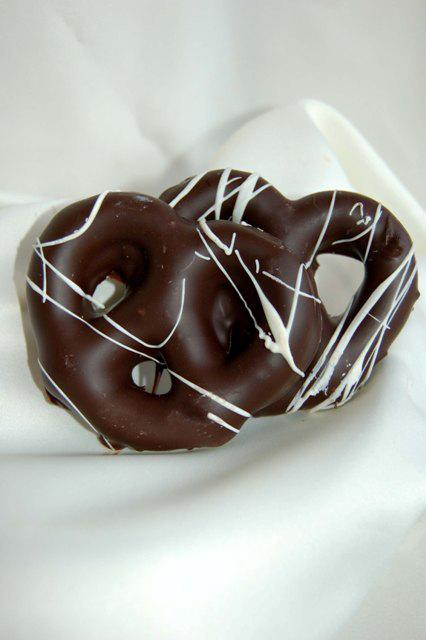
\includegraphics[width=6.0cm, trim=0 150 0 150, clip]{figures/donut_q75.jpeg}}
		\centerline{(1a) Q=75}
%		\centerline{Face++ prediction=["donut"]}
		\centerline{Face++ prediction \ = \ ["donut"]}
		\vspace{0.4cm}
	\end{minipage}
	\hfill
	\begin{minipage}{0.5\linewidth}
		\centerline{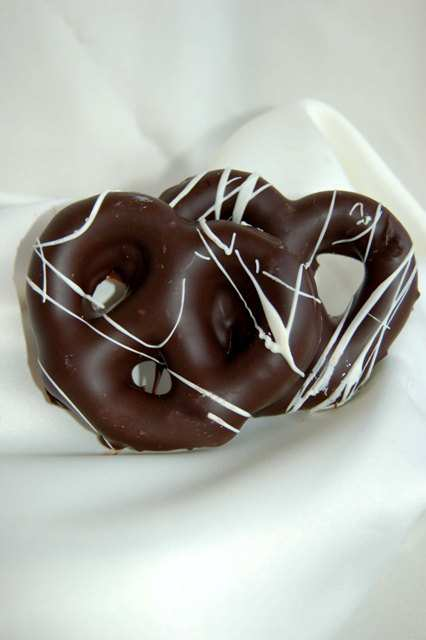
\includegraphics[width=6.0cm, trim=0 150 0 150, clip]{figures/donut_q55.jpeg}}
		\centerline{(1b) Q=55}
%		\centerline{Face++ prediction=[]}
		\centerline{Face++ prediction \ = \ ["biscuit"]}
		\vspace{0.4cm}
	\end{minipage}
	\vfill	
	\begin{minipage}{0.5\linewidth}
		\centerline{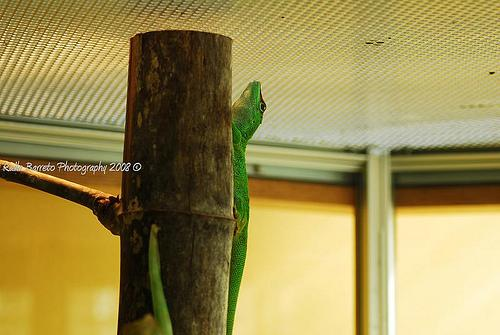
\includegraphics[width=6.0cm, trim=0 0 0 0]{figures/chameleon_q75.jpeg}}
		\centerline{(2a) Q=75}
% 		\centerline{\quad Baidu prediction=["chameleon"]}
		\centerline{Baidu prediction \ = \ ["chameleon"]}
		\vspace{0.4cm}
	\end{minipage}
	\hfill
	\begin{minipage}{0.5\linewidth}
		\centerline{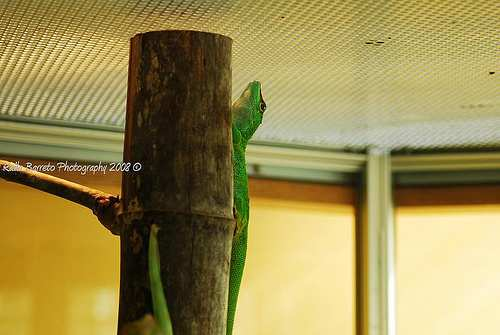
\includegraphics[width=6.0cm, trim=0 0 0 0]{figures/chameleon_q55.jpeg}}
		\centerline{(2b) Q=55}
% 		\centerline{\qquad Baidu prediction=["electric fan"]}
 		\centerline{Baidu prediction \ = \ ["electric fan"]}
 		\vspace{0.4cm}
	\end{minipage}
	\vfill
	\begin{minipage}{0.5\linewidth}
		\centerline{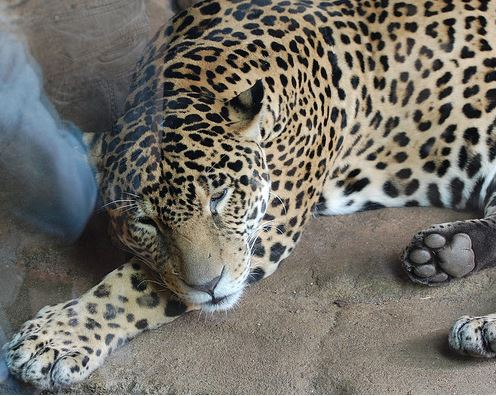
\includegraphics[width=6.0cm, trim=0 0 0 0, clip]{figures/tiger_highq.jpeg}}
		\centerline{(3a) Q=75}
%		\centerline{Baidu prediction=["leopard"]}
		\centerline{Baidu prediction \ = \ ["leopard"]}
		\vspace{0.3cm}
	\end{minipage}
	\hfill
	\begin{minipage}{0.5\linewidth}
		\centerline{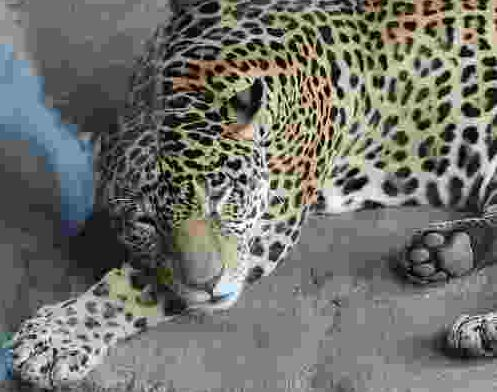
\includegraphics[width=6.0cm, trim=0 0 0 0, clip]{figures/tiger_lowq.jpeg}}
		\centerline{(3b) Q=5}
%		\centerline{Baidu prediction=["leopard"]}
		\centerline{Baidu prediction \ = \ ["leopard"]}
		\vspace{0.3cm}
	\end{minipage}
%	\end{tabular}
	\caption{The prediction of a deep learning model is not completely related to the input image's quality, making it difficult to use a fixed compression quality for all images. For image 1a, 1b and 2a, 2b, minor changes cause different predictions though they are visually similar; for image 3a and 3b, the cloud model still output correct label from a severely compressed image though they look very different}
	\label{fig: compress_accuracy}
%	\vspace{-0.1cm}
\end{figure*}

To address the above challenges, we present a reinforcement learning-based solution, called AdaCompress\footnote{We open-sourced AdaCompress that works with online computer vision-based APIs at \url{https://github.com/hosea1008/AdaCompress}}, to choose the proper compression quality level for an image to a computer vision model on the cloud, in an online manner. This paper is an extension of our earlier conference paper~\cite{2019adacompress}, with the following contributions:

$\rhd$ We design an interactive training environment that can be applied to different online computer vision-based services. We propose a Deep Q-learning Network-based~\cite{DQN} agent to evaluate and predict the performance of a compression quality level on an input image. In real-world application scenarios, this agent can be highly efficient to run on today's edge infrastructures (e.g., Google edge TPU~\cite{google-tpu}, Huawei Atlas 500 edge station~\cite{huawei-atlas500}).
	
$\rhd$ We build a reinforcement learning-based framework to train the agent in the above environment. The agent can learn to choose a proper compression quality level for an input image after iteratively interacting with the environment by feeding the carefully designed reward that considers both accuracy and data size. Based on~\cite{2019adacompress}, we further propose an \emph{explore-exploit} mechanism to let the agent switch between ``sceneries''. In particular, after deploying the agent, an \emph{inference-estimate-retrain} solution is designed to restart the training once the scenery changes and the existing running agent cannot guarantee the original accuracy performance.
	
$\rhd$~~In this journal extension, we provide more analysis and insights on our design. By analyzing the Deep Q-learning Network-based agent's behaviors using Grad-Cam~\cite{grad-cam}, we provide the reasons that the agent chooses a specific compression quality level. We reveal that images containing large smooth areas are more sensitive to compression, while images with complex textures are more robust to compression for computer vision models.
	
$\rhd$ We evaluate our system on representative cloud deep learning services, including Amazon Rekognition~\cite{amazon_rekognition}, Face++~\cite{face++_service} and Baidu Vision~\cite{baidu_vision}, and show that our design can reduce the upload traffic load by up to $1/2$ while maintaining comparable overall accuracy. Compared to baseline DeepN-JPEG~\cite{DeepN-JPEG}, the overall accuracy of AdaCompress is $8\%$ higher when they have similar compressed image size.

% \begin{itemize}
% 	\item First, we completed designing agent caching strategy work mentioned in our previous version's future work~\cite{2019adacompress}, adding the model query state in previous inference-estimate-retrain mechanism to avoid unnecessary upload traffic load in the retraining phase. Once capturing the scenery change, comparing to the previous mechanism that retrains from scratch directly, in our new mechanism, AdaCompress switches into model query state and loads a suitable RL agent model, achieving a lower upload traffic load. In the experiment, we use the FLIR Thermal Dataset instead of the previous DNIM Dataset to act as a nighttime scenery since thermal sensors capture gray-scaled thermal images in the nighttime, and the experiment result shows that our design can cut down the uploading file size overhead effectively.
% 	\item Second, for the comparison purpose, we implement the DeepN-JPEG framework according to~\cite{DeepN-JPEG} and evaluate the size reduction and accuracy performance. Our experiment shows that AdaCompress and DeepN-JPEG both decrease the uploading file size overhead more than 1/2, but the inference accuracy of AdaCompress is 8\% higher than that of DeepN-JPEG. Moreover, we provide illustrative image examples to present that AdaCompress compresses images more adaptively to achieve higher accuracy.
% 	\item Last but not least, we re-organize and amend the manuscript significantly to be easier to follow.
% \end{itemize}
The rest of this paper is organized as follows. We discuss related works in Sec.~\ref{sec: related_works}. In Sec.~\ref{sec: design} we present our framework and detailed design. We present our solution's performance in Sec.~\ref{sec: evaluation} and conclude the paper in Sec.~\ref{sec: conclusion}.

%The rest of this paper is organized as follows. We present our framework and detailed design in Sec.~\ref{sec: design}. In Sec.~\ref{sec: evaluation} we present our solution's performance. We discuss related works in Sec.~\ref{sec: related_works} and conclude the paper in Sec.~\ref{sec: conclusion}.
\section{Related Works}
\label{Section: related_works}

As online computer vision-based services have become the norm for today's applications~\cite{huynh2017deepmon, agrawal2015cloudcv}, many studies have been devoted to improving the cloud-based model execution, including model compression and data compression.

\subsection{Model Compression}

Though the accurate term is still for the community to debate, we use ``model compression'' to represent the studies on \emph{compressing} and \emph{moving} the deep learning models close to users. Many studies tried to compress the deep learning models and deploy them \emph{locally}~\cite{prun_quanti, pruning_han, quantize, quantize_3bit, quantization, structured_pruning}, i.e., running an alternative ``smaller version'' of a computer vision model at the user-side, to avoid the image upload so that to improve the inference efficiency. Other studies proposed to run a part of a deep learning model \emph{locally}~\cite{ILP_Decoupling, jalad, Edge_LBP, Neurosurgeon}, by decoupling the deep learning model into different parts, e.g., based on the layers in the deep learning model, so that a part of the inference is done \emph{locally} to save some execution time. However, these solutions usually need to re-train the model using the original dataset of the model, which is not practical for today's online computer vision-based services that are merely a black box to end-users, e.g., in the form of a RESTful API.

\subsection{Data Compression}

Data compression solutions study how to compress the original data (e.g., a video or image) to be inferred by the cloud-based deep learning model so that less traffic is used to upload the data to improve inference speed. In recent years, researchers found that conventional human visually optimized-based data compression solutions (e.g., JPEG~\cite{jpeg}, WebP~\cite{calore2010meet} and JPEG2000~\cite{rabbani2002jpeg2000}, etc.) and some recent neural network-based compression solutions~\cite{toderici2017full, theis2017lossy, toderici2015variable, rippel2017real} are not usually applicable to deep learning vision models. Liu et al.~\cite{DeepN-JPEG} revealed that the conventional JPEG image compression framework is designed for the Human-Visual System, which is not suitable for the deep neural network, leading to the computer vision model's inference performance degradation. Dodge et al.~\cite{dodge2016understanding} further discovered that besides the JPEG compression, four types of quality distortions (blur, noise, contrast, and the JPEG2000 compression~\cite{rabbani2002jpeg2000}) can also affect the inference performance of the deep learning models. Delac et al.~\cite{delac2005effects} observed that, in some cases, a high compression quality level does not always reduce the model inference accuracy. %% \\

Based on these insights, Robert et al.~\cite{torfason2018towards} tried to train the deep neural network from the compressed representations of an auto-encoder. Chao et al.~\cite{chao2011preserving} proposed using variable quantization, which is supported by the JPEG standard extension syntax~\cite{dis199110918} to compress the macroblocks in images. Furthermore, they~\cite{chao2013design} designed a quantization table based on the observed impact of scale-space processing on the discrete cosine transform (DCT) basis functions for JPEG images, achieving similar inference performance while reducing the image size overhead effectively. Liu et al.~\cite{DeepN-JPEG} proposed DeepN-JPEG that re-designs the quantization table by linking statistical information of defined features and defined quantization values so that the compressed image size is reduced for deep learning models. Chamain et al.~\cite{2019quannet} proposed a joint optimization of image classification network coupled with the image quantization, achieving image size reduction of JPGE2000~\cite{rabbani2002jpeg2000} encoded images. Recently, Lionel et al.~\cite{gueguen2018faster} presented a new type of neural network that infers directly from the discrete cosine transform coefficients in the middle of the JPEG codec. Baluja et al.~\cite{baluja2019task} proposed task-specific compression that compresses images based on the end-use of images. %% \\

However, such proposals all need one to understand the characteristics of the cloud-based deep learning model and have access to the original training dataset,  \emph{generating} the appropriate compression schemes. To the best of our knowledge, we are the first to propose an adaptive compression configuration solution that learns the optimal compression quality level to achieve an expected inference accuracy and upload image size, only from the online inference results, without knowing details of the model structures. 

In this journal extension, we improve the previous \emph{inference-estimate-retrain} mechanism to cut down the upload image size overhead effectively, add DeepN-JPEG comparative experiment, and amend the manuscript significantly. Especially in the DeepN-JPEG comparative experiment, since Liu et al.~\cite{DeepN-JPEG} evaluated the DeepN-JPEG framework on ImageNet by using four state-of-the-art DNN models (AlexNet~\cite{AlexNet-krizhevsky2012imagenet}, VGG~\cite{VGG-simonyan2014very}, GoogLeNet~\cite{GoogleNet-szegedy2015going} and ResNet~\cite{ResNet-he2016deep}) on local edge devices, which are different from online computer vision-based services, for comparison purpose, we implement the DeepN-JPEG framework according to their paper and evaluate the size reduction and accuracy performance using ImageNet and the metrics in Subsection~\ref{subsec:metrics} on three cloud-based deep learning services (Amazon Rekognition, Face++ and Baidu Vision).

%Liu et al.~\cite{DeepN-JPEG} developed the DeepN-JPEG framework, a deep %neural network favorable JPEG-based image compression framework.
\section{Detailed Design}
\label{Section: design}

\begin{figure*}[!t]
	%\begin{tabular}{cc}
	\begin{minipage}{\linewidth}
		\centerline{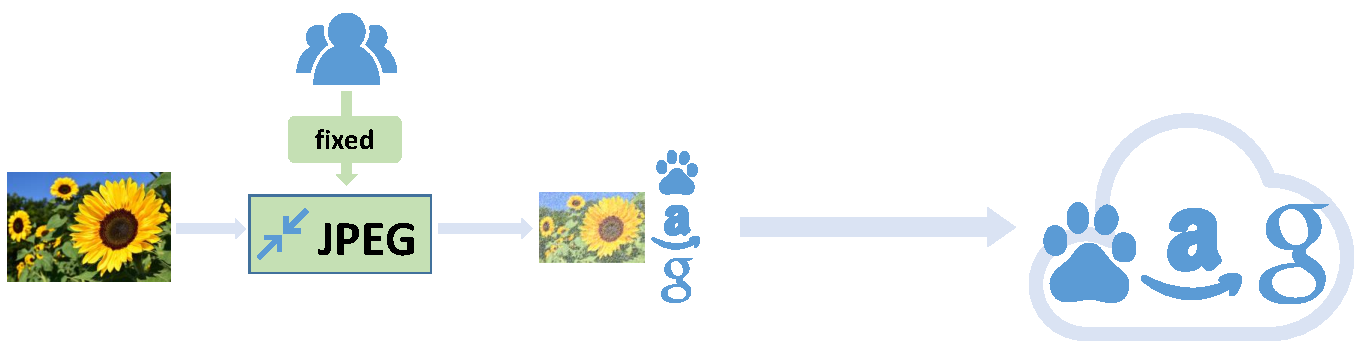
\includegraphics[width=0.8\linewidth]{figures/conventional-framework.pdf}}
		\begin{center}
			{(a) Conventional solution: fixed user-defined compression quality level}
		\end{center}
		%        \vspace{0.3cm}
	\end{minipage}
	\vfill
	\vspace{0.4cm}
	\begin{minipage}{\linewidth}
		\centerline{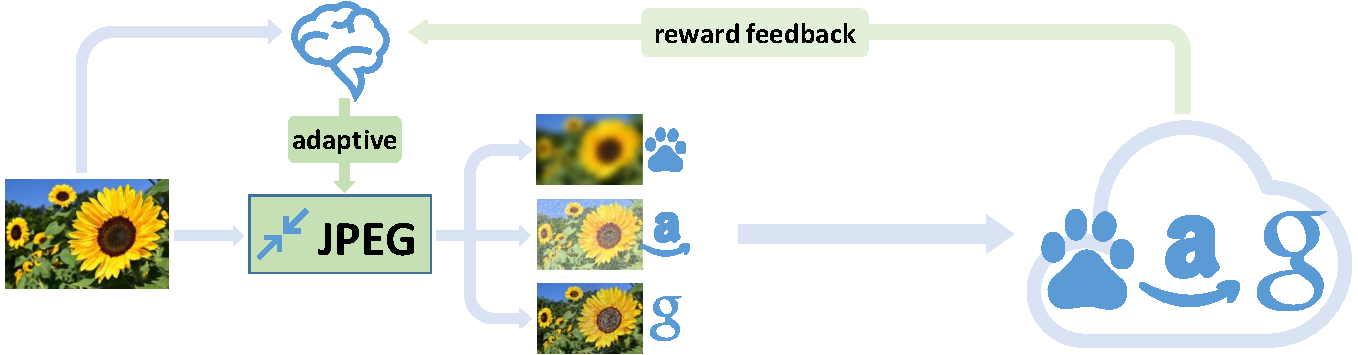
\includegraphics[width=0.8\linewidth]{figures/adaptive-framework.pdf}}
		\vspace{0.2cm}
		\begin{center}
			{(b) AdaCompress solution: input image and model aware compression}
		\end{center}
	\end{minipage}
	%\end{tabular}
	%\vspace{0.1cm}
	\caption{Comparing to the conventional solution, our solution can update the compression strategy based on the backend model feedback}
	\label{fig: framework}
\end{figure*}

A brief framework of AdaCompress is shown in Figure~\ref{fig: framework}. Briefly, it is a reinforcement learning-based system to train an agent to choose a proper compression quality level $ c $ for one image to be compressed by JPEG. We discuss the formulation, agent design, reinforcement learning-based framework, reward feedback, \emph{inference-estimation-querying-retraining} mechanism, and insight of RL agent's behaviors separately in the following subsections. We provide experimental details of all the hyperparameters in Section~\ref{Section: evaluation}. %% \\

\subsection{Problem Formulation}
\label{subsec: formulation}

% \colorbox{red}{notation table}
Without loss of generality, we denote the cloud-based deep learning service as $ \vec{y}_i = M(x_i) $ that provides a predicted result list $ \vec{y}_i $ for each input image $ x_i $. It has a baseline output $ \vec{y}_{\rm ref} = M(x_{\rm ref}) $ for each reference input image $ x \in X_{\rm ref} $. We use this $ \vec{y}_{\rm ref} $ as the ground truth label. For each image $ x_c $ compressed at compression quality level $ c $, the output $ \vec{y}_c = M(x_c) $. Therefore, we have an accuracy metric $ \mathcal{A}_c $ by comparing $ \vec{y}_{\rm ref} $ and $ \vec{y}_c $. In general, we use the top-5 accuracy as the following $ \mathcal{A} $, the same as the classification metric of ILSVRC2012~\cite{ILSVRC12}.

\begin{align}
\mathcal{A} =& \frac{1}{k} \sum_{k}\max_jd(l_j, g_k) \\
& l_j \in \vec{y}_c, \quad j=1,...,5 \\
& g_k \in \vec{y}_{\rm ref}, \quad k=1, ..., {\rm length}(\vec{y}_{\rm ref}) \\
& d(x, y) = 1 \ \text{if} \ x=y  \ \text{else} \ 0 
\end{align}

Where $ j = 1,...,5 $ indicates the prediction labels at the top-5 score, meaning that if any one of the top-5 predicted labels matches the ground truth label $ \vec{y}_{\rm ref} $, it would be regarded as a correct prediction. In general, we cannot get the cloud-based deep learning model's in-layer details (e.g., softmax probabilities) for a cloud-based deep learning service. Therefore we use a binary hard label $ d(x, y) \in \{0, 1\} $ to evaluate the accuracy. %% $ d(x, y) \in \{0, 1\} $

We also denote JPEG input images as $ f_{ic} = J(x_i, c) $ that for an input image $ x_i $ and a given compression quality level $ c $, and it outputs a compressed file $ f_{ic} $ at the size of {\color{revise2} $ \hat{s}_{ic} $}. For a reference compression quality level $ c_{\rm ref} $, the compressed file size is {\color{revise2} $ \hat{s}_{\rm ref} $}. Besides, the input image from a specific scenery usually belongs to a particular contextual group~\cite{mcdnn}. For example, in the daytime, the input images are expected to have a bright background, while nighttime images are usually gray-scaled thermal images. Therefore, the agent in one scenery does not need to know all the contextual features in all ``sceneries''. We formulate this as contextual group $ \mathcal{X} $.
%This contextual grouping concept is also discussed in~\cite{mcdnn}.

Initially, the agent tries different compression quality levels $ c_{\min} < c < c_{\max}, c \in \mathbb{N} $ to obtain compressed image $ x_c $ from input image $ x $. To obtain cloud-end recognition results $ \{\vec{y}_{\rm ref}, \vec{y}_c\} $, the agent uploads the compressed image $ x_c $ and the reference image $ x_{\rm ref} $ to the cloud-end. Comparing the two uploaded instances $ \{x_{\rm ref}, x_c\} $ and cloud-end recognition results $ \{\vec{y}_{\rm ref}, \vec{y}_c\} $, the agent obtains the reference file size {\color{revise2}$ \hat{s}_{\rm ref} $} and compressed file size {\color{revise2}$ \hat{s}_c $}, and computes the file compression ratio {\color{revise2}$ \Delta s = \frac{\hat{s}_c}{\hat{s}_{\rm ref}} $} and accuracy metric $ \mathcal{A}_c $.

\subsection{RL Agent Design}

The RL agent is expected to give a proper compression quality level $ c $ for minimizing the file size {\color{revise2}$ \hat{s}_c $} while keeping the accuracy $ \mathcal{A} $. {\color{revise2} In our design, each compression is treated as a complete RL task that only has one step, and the agent performs the action only once to accomplish the task. The agent is able to learn across consecutive tasks, because the input sequence (i.e., consecutive images likely to be captured by the same camera) shares similar contextual characteristics. The similar design has also been used in previous studies, including RL-based cache strategy \cite{wang2020intelligent_RL,zhong2018deep_RL,sadeghi2019deep_RL}.} For the RL agent, the input features are continuous numerical vectors, and the expected output is discrete compression quality level $ c $. Therefore we can use the Deep Q-learning Network as the RL agent. But the naive Deep Q-learning Network can not work well in this task because of the following challenges: %% \\

\begin{itemize}
	\item The state space of reinforcement learning is too large. To preserve enough details, we have to add many layers and nodes to the neural network, making the RL agent extremely difficult to converge. 
	\item It takes a long time to train one step in a large inference neural network, making the training process too time-consuming.
	\item The RL agent starts training from random trials and learns afterward from the reward feedback. When training from a randomly initialized neural network, the reward feedback is very sparse, making it difficult for the agent to learn.
\end{itemize}

To address these challenges, we use the early layers of a pre-trained neural network to extract the structural information of an input image. This is a commonly used strategy in training a deep neural network~\cite{finetunning,finetunning2}. Therefore instead of training a RL agent directly from the input image, we use a pre-trained small neural network to extract the features from the input image to reduce the input dimension and accelerate the training procedure. In this work, we use the early convolution layers of MobileNetV2~\cite{MobileNetV2} as the image feature extractor $ \mathcal{E}(\cdot) $ for its efficiency in image classification. The Deep Q-learning Network $ \phi $ is connected to the feature extractor's last convolution layer. We update the RL agent's policy by changing the parameters of the Deep Q-learning Network $ \phi $ while fixing the feature extractor $ \mathcal{E} $. %% \\

\subsection{Reinforcement Learning-based Framework}

In a specific scenery where the user input image $ x $ belongs to the contextual group $ \mathcal{X} $, we define the contextual group $ \mathcal{X} $, along with the backend cloud model $ M $, as the \emph{emulator environment} $ \{\mathcal{X}, M\} $ of the reinforcement learning problem. 

We formulate the feature extractor's output {\color{revise2} $ s = \mathcal{E}(J(\mathcal{X}, c)) $} \iffalse $ \mathcal{E}(J(\mathcal{X}, c)) $ \fi as \emph{states} and the compression quality level $ c $ as discrete \emph{actions}. In our system, to accelerate training, we define 10 discrete actions to indicate 10 compression quality levels of JPEG ranging from $ 5, 15, ...,95 $. We denote the \emph{action-value function} as {\color{revise2} $ Q(\mathcal{E}(f_t), c; \theta) $} \iffalse $ Q(\phi(\mathcal{E}(f_t)), c; \theta) $ \fi and the optimal compression quality level at time $ t $ as {\color{revise2} $  c_t = {\rm argmax}_cQ(\mathcal{E}(f_t), c; \theta) $} \iffalse $ c_t = {\rm argmax}_cQ(\phi(\mathcal{E}(f_t)), c; \theta) $ \fi where $ \theta $ indicates the parameters of the Deep Q-learning Network $ \phi $. In such reinforcement learning formulation, the training phase is to minimize the loss function $ L_i(\theta_i) = \mathbb{E}_{s, c \sim \rho (\cdot)}\Big[\big(y_i - Q(s, c; \theta_i)\big)^2 \Big] $ that changes at each iteration $ i $ where {\color{revise2} state $ s = \mathcal{E}(f_i) $} and target $ y_i = \mathbb{E}_{s' \sim \{\mathcal{X}, M\}} \big[ r + \gamma \max_{c'} Q(s', c'; \theta_{i-1}) \mid s, c \big] $. Especially, $ r $ is the reward feedback, and $ \rho(s, c) $ is a probability distribution over {\color{revise2} state} \iffalse sequences \fi $ s $ and the compression quality level $ c $~\cite{DQN}. When minimizing the distance of \emph{action-value function}'s output $ Q(\cdot) $ and target $ y_i $, the \emph{action-value function} $ Q(\cdot) $ outputs a more accurate estimation of an action. 

Different from conventional reinforcement learning, the interactions between the agent and environment are infinite, i.e., there is no signal from the environment telling that an episode has finished. Therefore, we train the RL agent intermittently at a manual interval of $ T $ after the condition $ t \geq T_{\rm start} $ guaranteeing that there are enough transitions in the memory buffer $ \mathcal{D} $. In the training phase, the RL agent firstly takes some random trials to observe the environment's reaction and decreases the randomness when training afterward. {\color{revise2} In iteration t, we  leverage the feature extractor $\mathcal{E}$ to obtain state $s_t = \mathcal{E}(J(x_t,c_{ref}))$. The RL agent $\phi$ generates a compresion quality level $c_t$. The framework compresses image $x_t$ at quality $c_t$ to upload and obtains reward $r_t$. The framework obtains next image $x_{t+1}$ and generates next state $ s_{t+1} = \mathcal{E}\big(J(x_{t+1},c_{ref})\big) $. The framework stores transition $(s_t, c_t, r_t, s_{t+1},\mathcal{A}_t )$ in a memory buffer $\mathcal{D}$. Especially, $(s_t, c_t, r_t, s_{t+1} )$ is uesd to compute the loss function, and $(r_t,\mathcal{A}_t )$ is used in \ref{subsec: mechanism}  Inference-Estimation-Querying-Retraining Mechanism.} All transitions are saved into a memory buffer $ \mathcal{D} $, and the agent learns to optimize its \emph{action} by minimizing the loss function $ L $ on a mini-batch from $ \mathcal{D} $. The training procedure would converge when the agent's randomness keeps decaying. Finally, the agent's action is based on its historical ``optimal'' experiences. The training procedure is presented in Algorithm~\ref{alg: rl-train}.
% and we list the parameters in Section.~\ref{Section: evaluation}.


\begin{algorithm}[!t]
{\color{revise2}
	\caption{Training RL agent $ \phi $ in environment $ \{\mathcal{X}, M\} $}
	\label{alg: rl-train}
	\begin{algorithmic}[1]
		\STATE Initialize replay memory buffer $ \mathcal{D} $ to capacity $ N $
		\STATE Initialize \emph{action-value function} $ Q $ with random weights $ \theta $
		{\color{revise2}
		\STATE Initialize state $ s_1 \leftarrow \mathcal{E}\big(J(x_1, c_{ref})\big), x_1 \in \mathcal{X} $ }
%		and $ \phi_1 = \phi(f_1) $
		\FOR {$t \in 1,2,\cdots, K$}
%		\STATE \textbf{1) Exploration.} %With probability $\epsilon$:
		\STATE \textbf{1) Exploration}
		\STATE With probability $\epsilon$:
		\STATE \hspace{1em} $c_t \leftarrow$ a random valid value 
		\STATE Otherwise:
		{\color{revise2}
		\STATE \hspace{1em} $ c_t \leftarrow {\rm argmax}_cQ(\mathcal{E}(f_t), c; \theta) $ }
%		{\rm argmax}_cQ\Big(\big(\mathcal{E}(f_t)\big), c; \theta\Big) $
		\STATE
		
%		\STATE \textbf{2) Reward calcuation.} 
		\STATE \textbf{2) Reward calcuation} 
		\STATE Compress image $ x_t $ at quality $ c_t $ to upload
		\STATE Receive $ (\vec{y}_{\rm ref}, \vec{y}_c) $ from the cloud service
		{\color{revise2} \STATE Compute reward $ r \leftarrow R(\Delta s, \mathcal{A}_c) $ according to \ref{subsec: reward} Reward Feedback Design}
		
		\STATE 
%		\STATE \textbf{3) Gradient decent.} %Generate $ c_t, x_{t+1} $
		\STATE \textbf{3) Gradient descent}
		{\color{revise2}\STATE Obtain next image $ x_{t+1} $
		\STATE Generate next state $ s_{t+1} \leftarrow \mathcal{E}\big(J(x_{t+1},c_{ref})\big) $
%		, $ \phi_{t+1} \leftarrow \phi \big(\mathcal{E}(f_{t+1})\big) $
%		\STATE $ s_{t+1} \leftarrow s_t $, $ \phi_{t+1} \leftarrow \phi \big(\mathcal{E}(f_{t+1})\big) $
		\STATE $ \mathcal{D} \leftarrow \mathcal{D} \bigcup \{(s_t, c_t, r_t, s_{t+1},\mathcal{A}_t ) \} $
%		\STATE $ \mathcal{D} \leftarrow \mathcal{D} \bigcup \{(\phi_t, c_t, r_t, \phi_{t+1}) \} $
		\IF {$ t \mod T = 0 $ and $ t \geq T_{\rm start} $}
%		\STATE Sample a randomly mini-batch of transitions \\ $ (\phi_j, c_j, r_j, \phi_{j+1}) $ from memory buffer $ \mathcal{D} $
		\STATE Sample a randomly mini-batch of transitions $ (s_j, c_j, r_j, s_{j+1},\mathcal{A}_j ) $ from memory buffer $ \mathcal{D} $
		\STATE $ y_j \leftarrow r_j + \gamma \max_{c'}Q(s_{j+1}, c'; \theta) $
		\STATE Compute decay exploration rate 
		$ \epsilon \leftarrow 
		\begin{cases}
		\mu_{\rm dec}\cdot \epsilon & \text{ if } \ \mu_{\rm dec}\cdot \epsilon > \epsilon_{\min} \\ 
		\epsilon_{\min}             & \text{ if } \ \mu_{\rm dec}\cdot \epsilon \leq \epsilon_{\min}
		\end{cases} $
		\STATE Perform a gradient descent step on $ \big(y_j - Q(s_j, c_j; \theta)\big)^2 $ according to~\cite{DQN}
		
%		\STATE Perform a gradient descent step on \\ $ \big(y_j - Q(\phi_j, c_j; \theta)\big)^2 $ according to~\cite{DQN}
		\ENDIF
	    }
		\ENDFOR
	\end{algorithmic}
}
\end{algorithm}


%\begin{algorithm}[!t]
%	\caption{Training RL agent $ \phi $ in environment $ \{\mathcal{X}, M\} $}
%	\label{alg: rl-train}
%	\begin{algorithmic}[1]
%		\STATE Initialize replay memory buffer $ \mathcal{D} $ to capacity $ N $
%		\STATE Initialize \emph{action-value function} $ Q $ with random weights $ \theta $
%		\STATE Initialize sequence $ s_1 = \mathcal{E}\big(J(x_1, c_1)\big), x_1 \in \mathcal{X} $ and $ \phi_1 = \phi(f_1) $
%		\FOR {$t \in 1,2,\cdots, K$}
%		%		\STATE \textbf{1) Exploration.} %With probability $\epsilon$:
%		{\color{revise}\STATE \textbf{1) Exploration}}
%		{\color{revise}\STATE With probability $\epsilon$:}
%		\STATE \hspace{1em} $c_t \leftarrow$ a random valid value 
%		\STATE Otherwise:
%		\STATE \hspace{1em} $ c_t \leftarrow {\rm argmax}_cQ\Big(\phi\big(\mathcal{E}(f_t)\big), c; \theta\Big) $
%		
%		\STATE
%		
%		%		\STATE \textbf{2) Reward calcuation.} 
%		{\color{revise}\STATE \textbf{2) Reward calcuation}} 
%		\STATE Compress image $ x_t $ at quality $ c_t $ to upload
%		\STATE Receive $ (\vec{y}_{\rm ref}, \vec{y}_c) $ from the cloud service
%		\STATE $ r \leftarrow R(\Delta s, \mathcal{A}_c) $
%		
%		\STATE 
%		%		\STATE \textbf{3) Gradient decent.} %Generate $ c_t, x_{t+1} $
%		{\color{revise}\STATE \textbf{3) Gradient decent}}
%		{\color{revise}\STATE Generate $ c_t, x_{t+1} $}
%		\STATE $ s_{t+1} \leftarrow s_t $, $ \phi_{t+1} \leftarrow \phi \big(\mathcal{E}(f_{t+1})\big) $
%		\STATE $ \mathcal{D} \leftarrow \mathcal{D} \bigcup \{(\phi_t, c_t, r_t, \phi_{t+1}) \} $
%		\IF {$ t \mod T = 0 $ and $ t \geq T_{\rm start} $}
%		%		\STATE Sample a randomly mini-batch of transitions \\ $ (\phi_j, c_j, r_j, \phi_{j+1}) $ from memory buffer $ \mathcal{D} $
%		{\color{revise}
%			\STATE Sample a randomly mini-batch of transitions $ (\phi_j, c_j, r_j, \phi_{j+1}) $ from memory buffer $ \mathcal{D} $
%			\STATE $ y_i \leftarrow r_j + \gamma \max_{c'}Q(\phi_{j+1}, c'; \theta) $
%			\STATE Compute decay exploration rate 
%			$ \epsilon \leftarrow 
%			\begin{cases}
%			\mu_{\rm dec}\cdot \epsilon & \text{ if } \ \mu_{\rm dec}\cdot \epsilon > \epsilon_{\min} \\ 
%			\epsilon_{\min}             & \text{ if } \ \mu_{\rm dec}\cdot \epsilon \leq \epsilon_{\min}
%			\end{cases} $
%			\STATE Perform a gradient descent step on $ \big(y_j - Q(\phi_j, c_j; \theta)\big)^2 $ according to~\cite{DQN}
%		}
%		%		\STATE Perform a gradient descent step on \\ $ \big(y_j - Q(\phi_j, c_j; \theta)\big)^2 $ according to~\cite{DQN}
%		\ENDIF
%		\ENDFOR
%	\end{algorithmic}
%\end{algorithm}

\subsection{Reward Feedback Design}
\label{subsec: reward}

In our solution, the agent is trained by the reward feedback from the environment $ \{\mathcal{X}, M\} $. In the above formulation, we define compression rate {\color{revise2}$ \Delta s = \frac{\hat{s}_c}{\hat{s}_{\rm ref}} $} \iffalse $ \Delta s = \frac{s_c}{s_{\rm ref}} $ \fi and accuracy metric $ \mathcal{A}_c $ at compression quality level $ c $. Basically, we want the agent to choose a proper compression quality level for minimizing the upload image size while remaining acceptable accuracy. \textcolor{revise}{Therefore the overall reward $ r $ should be positively correlated with the accuracy $ \mathcal{A} $ while negatively with the compression ratio $ \Delta s $.} We introduce two linear factors $ \alpha $ and $ \beta $ to form a linear combination $ r = \alpha \mathcal{A} - \Delta s + \beta $ as the \emph{reward function} $ R(\Delta s, \mathcal{A}) $. %% \\

% Therefore the overall reward $ r $ should be in proportion to the accuracy $ \mathcal{A} $ while in inverse proportion to the compression ratio $ \Delta s $.
\subsection{Inference-Estimation-Querying-Retraining Mechanism}
\label{subsec: mechanism}
As a running system, we introduce an \emph{inference-estimation-querying-retraining} mechanism to cope with the scenery change in the inference phase, building a system with different components to inferring, capturing the scenery change, then either re-loading or re-training the RL agent based on the performance of the cached model. The overall system diagram is illustrated in Figure~\ref{fig: diagram}.

%\begin{figure}[H]
%    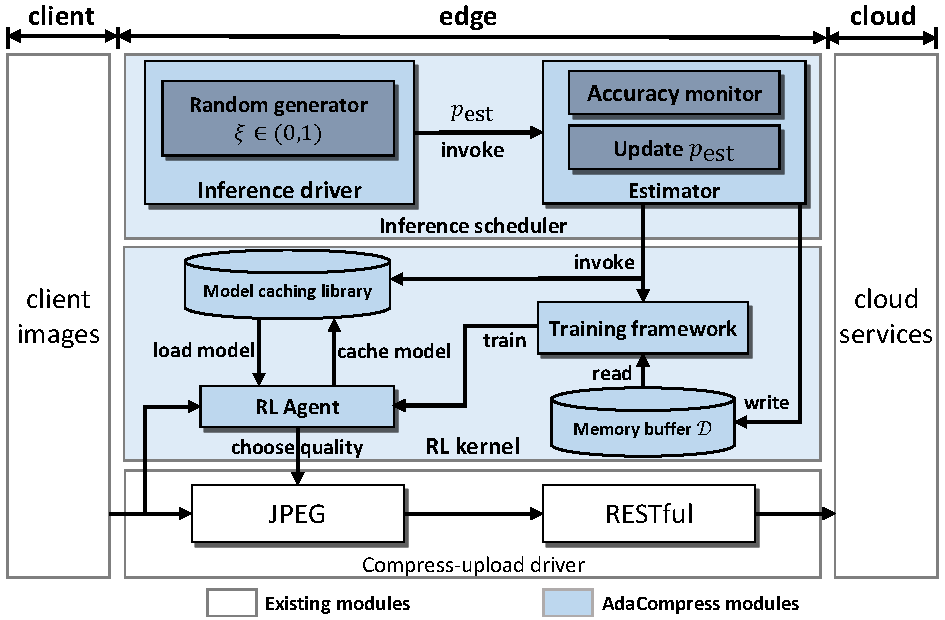
\includegraphics[width=\linewidth]{figures/overall-diagram.pdf}
%    \caption{Diagram of AdaCompress architecture}
%    \label{fig: diagram}
%\end{figure}

\begin{figure}[!t]
	\centerline{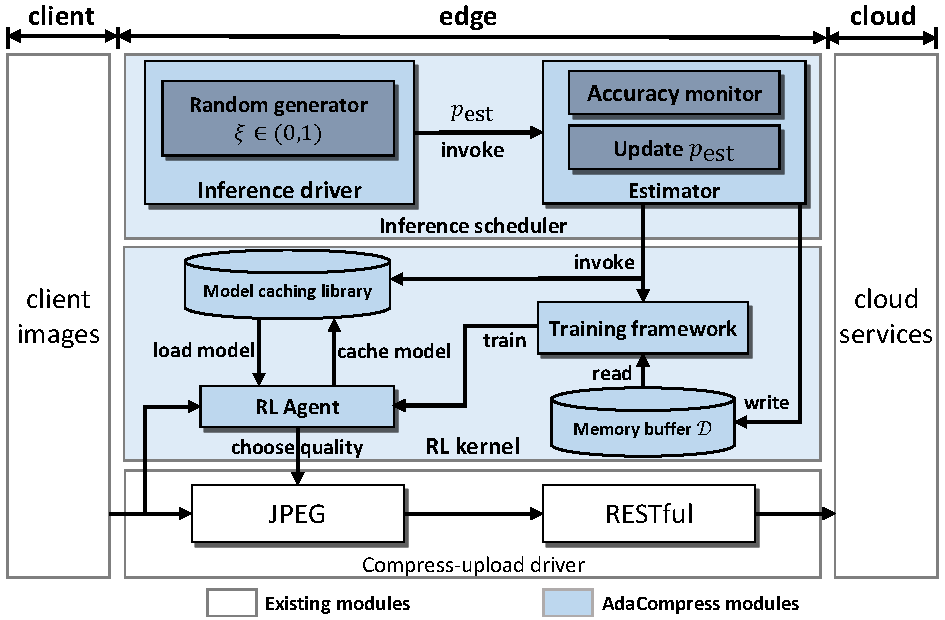
\includegraphics[width=0.8\linewidth]{figures/overall-diagram.pdf}}
%	\vspace{0.2cm}
	\caption{Diagram of AdaCompress architecture}
	\label{fig: diagram}
\end{figure}

%\begin{figure}[H]
%	\centerline{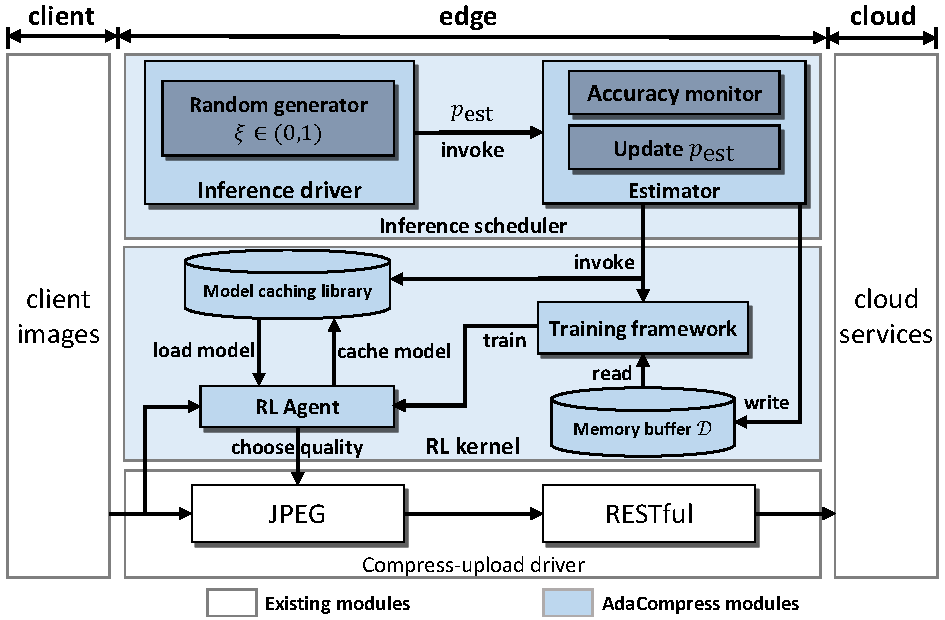
\includegraphics[width=0.8\linewidth]{figures/overall-diagram.pdf}}
%	\vspace{0.2cm}
%	\caption{Diagram of AdaCompress architecture}
%	\label{fig: diagram}
%\end{figure}

%% The system diagram is shown in Figure~\ref{fig: diagram}.
We build up the memory buffer $ \mathcal{D} $ and reinforcement learning training kernel based on the compression and upload driver. When the RL training kernel is called, it would load transitions from the memory buffer $ \mathcal{D} $ to train the compression quality level predictor $ \phi $. When the system is deployed, the pre-trained RL agent $ \phi $ guides the compression driver to compress the input image at an adaptive compression quality level $ c $, then uploads the compressed image to cloud-end. %% \\

After the AdaCompress is deployed, the input image scenery context $ \mathcal{X} $ may change (e.g., day to night, sunny to rainy). When the scenery changes, the older RL agent's compression selection strategy may not be suitable anymore, causing the overall accuracy to decrease. To cope with the scenery change, AdaCompress invokes an estimator with a probability $ p_{\rm est} $. AdaCompress does this by generating a random value $ \xi \in (0,1) $ and comparing it to $ p_{\rm est} $. If $ \xi \leq p_{\rm est} $, the estimator would be invoked. AdaCompress would upload the reference image $ x_{\rm ref} $ along with the compressed image $ x_i $ to obtain $ \vec{y}_{\rm ref} $ and $ \vec{y}_i $, calculate $ \mathcal{A}_i $ and save the transition {\color{revise2}$ (s_i, c_i, r_i, s_{i+1},\mathcal{A}_i ) $} \iffalse $ (\phi_i, c_i, r_i, \mathcal{A}_i) $ \fi to the memory buffer $ \mathcal{D} $. The estimator also compares the recent $ n $ steps' average accuracy $ \bar{\mathcal{A}}_n $ and the initial accuracy threshold $ \mathcal{A}_0 $. Once the recent average accuracy is lower than the initial accuracy threshold, the estimator would query a RL agent model to replace the current agent model and test the performance of the loaded model. To test the loaded model's performance, the estimator computes the average accuracy $ \bar{\mathcal{A}}^*_n $. If $ \bar{\mathcal{A}}^*_n $ is still lower than the accuracy threshold, the estimator would invoke the RL training kernel to re-train the agent. Once the estimator discovers that the trained reward is higher than the reward threshold, it would stop the training kernel, cache the trained RL agent, and switch to the normal inference state. 

Since the reference image $ x_{\rm ref} $ and the compressed image $ x_i $ are both needed in the re-training phase, causing a large upload image size overhead, especially when the scenery changes frequently (e.g., day to night, then night to day). To avoid unnecessary upload traffic load in the re-training phase, we build up the model caching library to cache the trained RL agent models. When capturing the scenery change, we firstly query a pre-trained model from the model caching library rather than re-training from scratch. %% \\

The \emph{inference-estimation-querying-retraining} mechanism has four states, including inference, estimation, model querying and re-training. AdaCompress switches to these states adaptively. The state switching policy is shown as Figure~\ref{fig: state-switching}.
%\begin{figure}[H]
%    \begin{tikzpicture}[->,>=stealth',shorten >=1pt,auto,node distance=1.8cm, semithick]
%    \tikzstyle{every state}=[ellipse, align=center, draw=blue, text=black]
%    
%    \node[initial, state] (B)                    {inference};
%    \node[state]         (C) [below right of=B] {re-train};
%    \node[state]         (D) [above right of=C] {estimate};
%    
%    \path   (B) edge [loop above] node {$ \xi > p_{\rm est} $} (B)
%    (B.10)    edge                node {$ \xi \leq p_{\rm est} $} (D.170)
%    (C) edge [below left]      node {$ \bar{r}_n > r_{\rm th} $} (B)
%    edge [loop below] node {$ \bar{r}_n \leq r_{\rm th} $}     (C)
%    (D) edge [loop right] node {$ \xi \leq p_{\rm est} $} (D)
%    (D.190)    edge              node {$ \xi > p_{\rm est} $} (B.-10)
%    (D.225)    edge [below right]      node {$ \bar{\mathcal{A}_n} < \mathcal{A}_0 $} (C);
%    \end{tikzpicture}
%    % \vspace{-0.3cm}
%    \caption{State switching policy}
%    \label{fig: state-switching}
%    %\vspace{-0.8cm}
%\end{figure}
\begin{figure}[!t]
	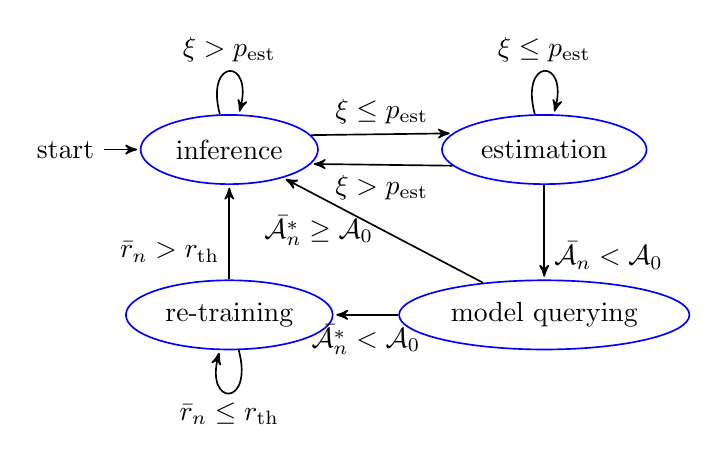
\begin{tikzpicture}[->,>=stealth',shorten >=1pt,auto,node distance=2.1cm, semithick]
	\tikzstyle{every state}=[ellipse, align=center, draw=blue, text=black]
	
	\node[initial, state] (B)                    {inference};
	\node[state]         (C) [below of=B] {re-training};
	\node[state]         (D) [right of=B, node distance=4cm] {estimation};
	\node[state]         (E) [right of=C, node distance=4cm] {model querying};
	%    \node[state][rectangle]   (F) [below right of=C, node distance=2.5cm] {Model Library};
	
	\path   (B) edge [loop above] node {$ \xi > p_{\rm est} $} (B)
	(B.10)    edge                node {$ \xi \leq p_{\rm est} $} (D.170)
	(C) edge [below left]      node {$ \bar{r}_n > r_{\rm th} $} (B)
	edge [loop below] node {$ \bar{r}_n \leq r_{\rm th} $}     (C)
	(D) edge [loop above] node {$ \xi \leq p_{\rm est} $} (D)
	(D.190)    edge              node {$ \xi > p_{\rm est} $} (B.-10)
	(D)    edge [below right]      node {$ \bar{\mathcal{A}_n} < \mathcal{A}_0 $} (E)
	(E) edge [below left] node [left] {$ \bar{\mathcal{A}^*_n} \geq \mathcal{A}_0 $} (B)
	(E) edge [below left] node [below] {$ \bar{\mathcal{A}^*_n} < \mathcal{A}_0 $} (C);
	%    (C) edge [below right] node [left] {cache model} (F)
	%    (F) edge [below right] node [right] {load model} (E);
	\end{tikzpicture}
	% \vspace{-0.3cm}
	\caption{State switching policy}
	\label{fig: state-switching}
	%\vspace{-0.8cm}
\end{figure}

%\subsubsection{\textbf{Inference}}
\subsubsection{Inference:}

Most of the time, AdaCompress runs in this state. In this state, only the compressed images are uploaded to the cloud-end to achieve less upload image size overhead. To keep a stable accuracy performance even the input image scenery changes, the agent would occasionally switch to the estimation state with probability $ p_{\rm est} $ since the estimator uploads the reference image to maintain inference accuracy, or remain in the inference state with probability $ 1 - p_{\rm est} $. %% \\

%\subsubsection{\textbf{Estimation}}
\subsubsection{Estimation:}

In this state, the reference image $ x_{\rm ref} $ and compressed image $ x_i $ are uploaded to the cloud-end simultaneously to obtain $ \vec{y}_{\rm ref} $ and $ \vec{y}_i $ which are used to calculate $ \mathcal{A}_i $. In each epoch $ i $, the transition {\color{revise2}$ (s_i, c_i, r_i, s_{i+1},\mathcal{A}_i ) $} \iffalse $ (\phi_i, c_i, r_i, \mathcal{A}_i) $ \fi is logged in the memory buffer $ \mathcal{D} $. When the average accuracy $ \bar{\mathcal{A}}_n $ of the latest $ n $ steps is higher than the accuracy threshold $ \mathcal{A}_0 $, the agent would stay in the estimation state with probability $ p_{\rm est} $ or switch to the inference state with probability $ 1 - p_{\rm est} $. Once the average accuracy $ \bar{\mathcal{A}}_n $ is lower than the initial accuracy threshold $ \mathcal{A}_0 $, indicating that the current agent is no more suitable for the current input image scenery, AdaCompress would turn into the model querying state and re-load a new RL agent model from the model caching library. %% \\

Therefore, the estimation probability of $ p_{\rm est} $ is vital to the whole system. On the one hand, the estimator should be invoked occasionally to estimate the current agent's accuracy for capturing the scenery change on time. On the other hand, the estimator uploads the reference image along with the compressed image. Therefore, the upload image size overhead is greater than the conventional benchmark solution, causing a high upload traffic load. %% \\

To achieve trade-off between the risk of the scenery change and the objective of reducing upload traffic load, we design an accuracy-aware dynamic solution. We first define that after running for $ N $ steps, the average accuracy of recent $ n $ steps is: 

\begin{align*}
\bar{\mathcal{A}_n} &=
\begin{cases}
%\frac{1}{n}\sum_{i=N-n}^{N} \mathcal{A}_i & \text{ if } N \geq n \\ 
%\frac{1}{n}\sum_{i=1}^{n} \mathcal{A}_i & \text{ if } N < n 
{\color{revise}\frac{1}{n}\sum_{i=N-n+1}^{N} } \mathcal{A}_i & \text{ if } N \geq n \\ 
{\color{revise}\frac{1}{N}\sum_{i=1}^{N} }\mathcal{A}_i & \text{ if } N < n 
\end{cases}
\end{align*}

With this definition, \textcolor{revise}{the change of $ p_{\rm est} $ should be negatively correlated with} the gradient of $ \mathcal{A} $, meaning that when the recent accuracy decreases, the estimation probability $ p_{\rm est} $ would increase. We define that $ p'_{\rm est} = p_{\rm est} + \omega \nabla \bar{\mathcal{A}} $ where $ \omega $ is a \textcolor{revise}{negative} scaling factor. With this recursive formula, we have the general term of $p_{\rm est} = p_0 + \omega {\color{revise}\sum_{i=1}^{N}} \nabla \bar{\mathcal{A}_i} $ where $ p_0 $ is an initial estimation probability.

% an intuitive formulation of % is in inverse proportion of
% \sum_{i=0}^{N}

%\subsubsection{\textbf{Model Querying}}
\subsubsection{Model Querying:}

The model querying state is designed to cope with the scenery change before re-training. It re-loads a new RL agent model from the model caching library and tests whether the loaded agent model is suitable for the current scenery by re-calculating the average accuracy. If the new average accuracy $ \bar{\mathcal{A}}^*_n $ is higher than the accuracy threshold $ \mathcal{A}_0 $, indicating that the loaded agent model is suitable for the current scenery, AdaCompress would switch to the normal inference state and use the loaded agent model to infer. Otherwise, AdaCompress would switch to the re-training state and invoke the RL training kernel to re-train a new RL agent for the current scenery.

In this way, AdaCompress is capable to cope with the scenery change in a cached ``memory'' manner, avoiding re-training the agent model at every scenery change to cut down the upload image size overhead. However, the agent caching strategy would cause a little storage overhead on local edge devices.


%\subsubsection{\textbf{Re-training}}
\subsubsection{Re-training:}

This state is to adapt the agent to the current input image scenery by re-training it with the memory buffer $ \mathcal{D} $, which is similar to the training procedure. The re-training phase has finished upon the recent $ n $ steps' average reward $ \bar{r}_n $ is higher than the user-defined threshold $ r_{\rm th} $. And when the re-training procedure finishes, the memory buffer $ \mathcal{D} $ would be flushed, preparing to save new transitions for the re-training of a next scenery change. The trained RL agent model would be cached in the model caching library and be used to switch to the inference state.

\subsection{Insight of RL Agent's Behaviors}
\label{subsec:insight}

In the inference phase, the pre-trained RL agent chooses a proper compression quality level according to the input image's features and the backend service. The reference image is not uploaded to the cloud-end anymore; only the compressed image is uploaded. Therefore, the upload traffic load is reduced. We notice that the RL agent's behaviors are various for different input image ``sceneries'' and backend cloud services. Therefore we try to make further investigations by plotting the RL agent's ``attention map'' (i.e., visual explanations why the agent chooses a specific compression quality level). %% \\

%\subsubsection{\textbf{Compression Level Choice Variation}}
\subsubsection{Compression Quality Level Choice Variation:}

\textcolor{revise}{As shown in Figure~\ref{fig: quality_chosen}, we find that in different cloud-based application environments, the agent's chosen compression quality levels can be quite different. We compute the \emph{mean} and \emph{standard deviation} of compression quality levels. The mean is $33.4$, $24.7$ and $31.6$ on Baidu Vison, Face++ and Amazon Rekognition, respectively. For Face++, the \emph{mean} of compression quality levels is lower than that for Baidu Vision. The standard deviation is $22.77$, $19.19$ and $22.46$ on Baidu Vison, Face++ and Amazon Rekognition, respectively.} The ``optimal'' compression strategies are different for different backend cloud services. This variation is caused by the interaction between the agent and the backend cloud model in the training phase. Since the agent's training procedure is based on a specific backend cloud model $ M_1 $, for another backend cloud model $ M_2 $, the interaction between the agent and $ M_2 $ is quite different. Therefore the agent's best compression quality level selection presents variation for different backend cloud models.

%In our experiment, we find that in different cloud-based application environments, the agent's chosen compression quality levels can be quite different. As shown in Figure~\ref{fig: quality_chosen}, for Face++ and Amazon Rekognition, the agent's choices are concentrated at around $ c=15 $, but for Baidu Vision, the agent's selections are distributed more evenly.

\begin{figure*}[!t]
{\color{revise}
	\begin{minipage}[t]{0.32\linewidth}
		\centerline{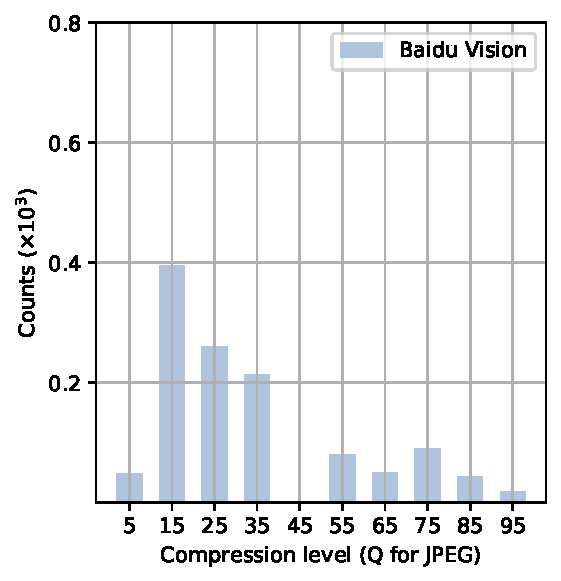
\includegraphics[width=4.8cm]{figures/ImageNet_Baidu_choices1.pdf}}
		\centerline{(a) Baidu Vision}
	\end{minipage}
	\hfill
	\begin{minipage}[t]{0.32\linewidth}
		\centerline{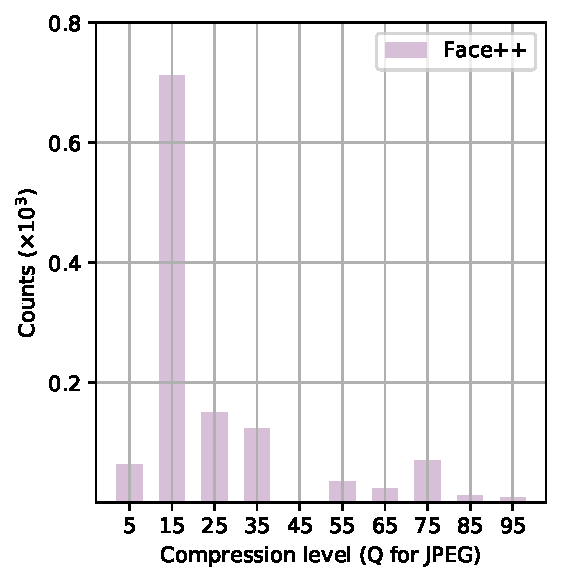
\includegraphics[width=4.8cm]{figures/ImageNet_Facepp_choices1.pdf}}
		\centerline{(b) Face++}
	\end{minipage}
	\hfill
	\begin{minipage}[t]{0.32\linewidth}
		\centerline{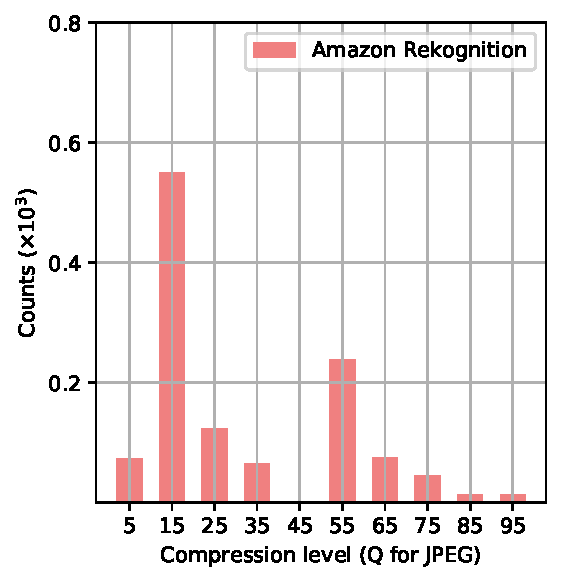
\includegraphics[width=4.8cm]{figures/ImageNet_Amazon_choices1.pdf}}
		\centerline{(c) Amazon Rekognition}
	\end{minipage}		
	\caption{\textcolor{revise}{Histogram of RL agent's best compression quality level selection for different cloud services}}
	\label{fig: quality_chosen}
}
\end{figure*}

%\begin{figure}[!t]
%	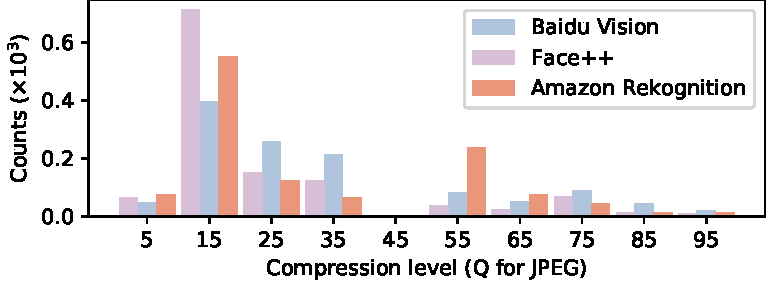
\includegraphics[width=0.8\linewidth]{figures/quality_chosen.pdf}
%	\caption{Histogram of RL agent's best compression quality level selection for different cloud services}
%	\label{fig: quality_chosen}
%	% \vspace{-0.3cm}
%\end{figure}

Moreover, in our experiment, the agent presents different behaviors when the input image changes from one dataset to another. Figure~\ref{fig: dataset_change} shows the agent's choices for the same backend cloud model (Baidu Vision) but different image datasets. We prepare two datasets indicating two contextual ``sceneries''. We randomly sample images from ImageNet~\cite{ImageNet} whose images are mostly taken in the daytime, to act as a daytime scenery, and randomly select nighttime images from the FLIR Thermal Dataset~\cite{FLIR} to form another dataset to act as a nighttime scenery. \textcolor{revise}{The histogram shown in Figure~\ref{fig: dataset_change} points out that the distribution of compression quality levels is different on ImageNet and FLIR Thermal Dataset. For ImageNet and FLIR, the mean is 43.3 and 47.5, respectively; and the standard deviation is 19.52 and 26.56, respectively.} To maintain high accuracy when the input image's contextual group $ \mathcal{X} $ changes, the agent's compression quality level selection should change as well. This phenomenon presents that the agent can adaptively choose a proper compression quality level based on the input image's features.

\textcolor{revise}{We can also find that Figure~\ref{fig: quality_chosen}(a) and Figure~\ref{fig: dataset_change}(a) is different, even if we use the same cloud service (Baidu Vision) and image dataset (ImageNet). When we use the same cloud service at different times, the cloud service commonly invokes different backend cloud models. Therefore the interaction between the agent and the backend cloud model is different. This variation presents that the agent can adaptively make a proper compression strategy in different complex environments, indicating our solution's generality and practicality.} %% \\

%The histogram shown in Figure~\ref{fig: dataset_change} points out that, for the ImageNet images, the agent prefers a low compression quality level, but its choices are distributed more evenly. For the FLIR Thermal images, the agent's choices are more accumulated in some relatively higher compression quality levels.

%\begin{figure}[!t]
%    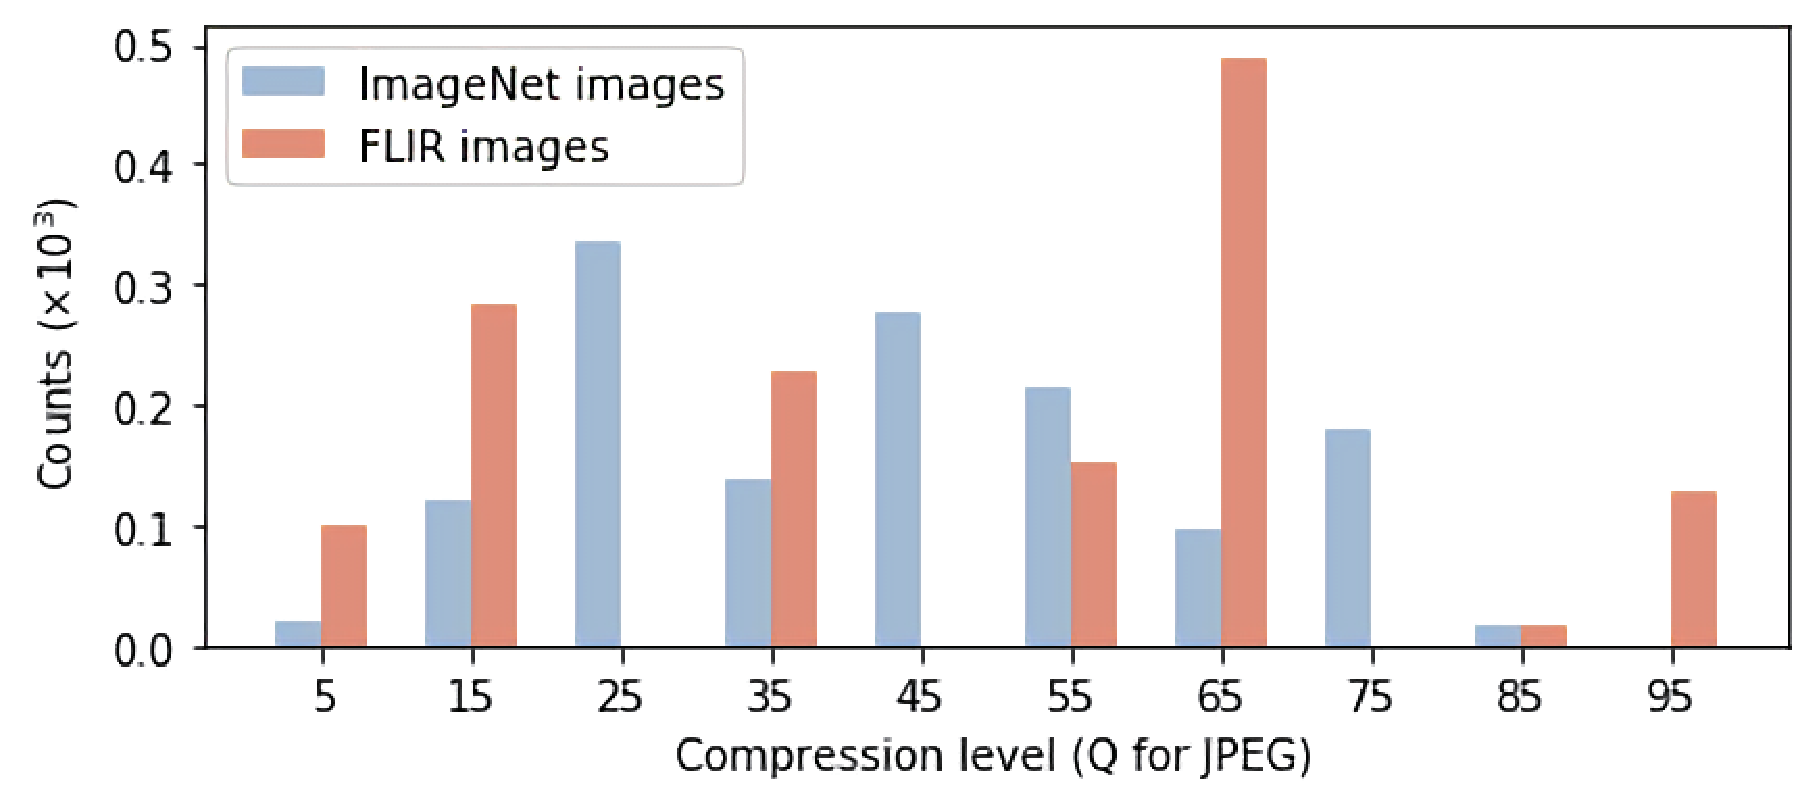
\includegraphics[width=0.8\linewidth]{figures/dataset_change.pdf}
%    \caption{Histogram of RL agent's best compression level selection for different scenery image inputs}
%    \label{fig: dataset_change}
%\end{figure}

\begin{figure*}[!t]
{\color{revise}
	\begin{minipage}[t]{0.48\linewidth}
		\centerline{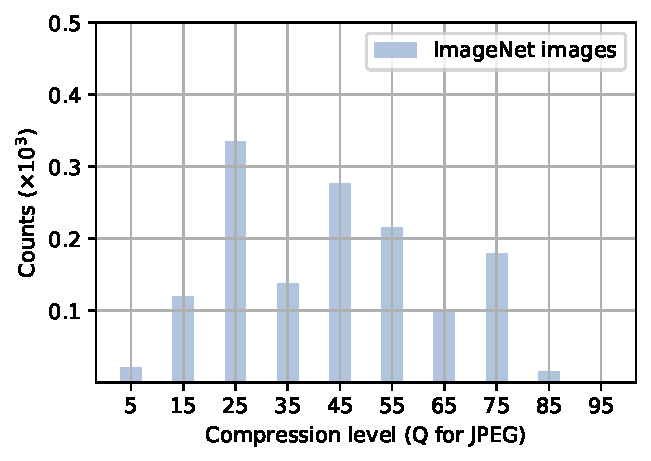
\includegraphics[width=7cm]{figures/ImageNet_Baidu_choices.pdf}}
		\centerline{(a) ImageNet images}
	\end{minipage}
	\hfill
	\begin{minipage}[t]{0.48\linewidth}
		\centerline{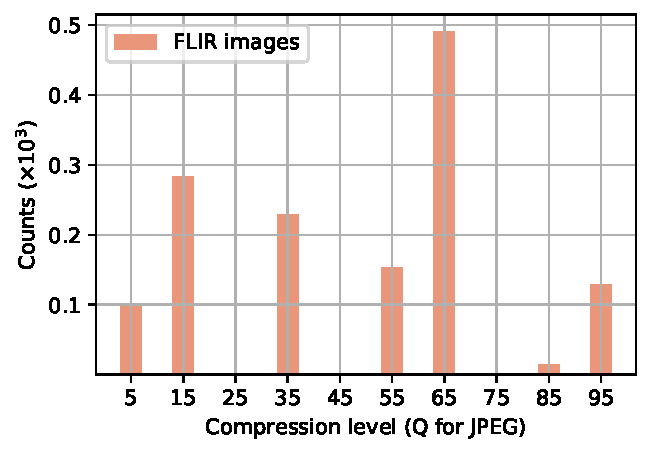
\includegraphics[width=7cm]{figures/FLIR_Baidu_choices.pdf}}
		\centerline{(b) FLIR images}
	\end{minipage}	
    \caption{\textcolor{revise}{Histogram of RL agent's best compression quality level selection for different scenery image inputs}}
	\label{fig: dataset_change}
}
\end{figure*}

%\subsubsection{\textbf{Attention Map Variation}}
\subsubsection{Attention Map Variation:}
\label{subsec: attention map}

To make insight investigations, we plot the importance map of a chosen compression quality level. We leverage a conventional visualization algorithm, Grad-Cam, to observe the Deep Q-Learning Network-based agent's interest when choosing compression quality levels. Grad-Cam is a widely used effective solution to present the importance map of a deep neural network by calculating the gradients of each target concept and backtracking to the final convolution layer. In this work, we plot the RL agent's attention map by Grad-Cam in Figure~\ref{fig: attention}. %% \\

\begin{figure*}[!t]
	\begin{minipage}{0.2\linewidth}
		\centerline{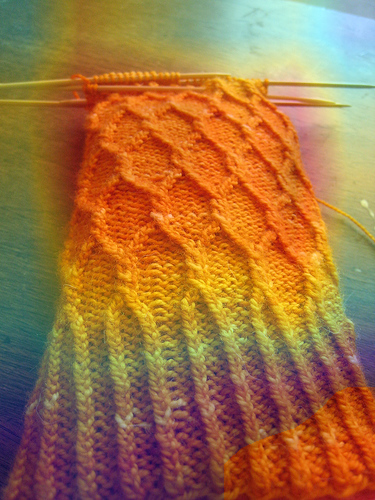
\includegraphics[width=3.5cm, height=3.0cm]{figures/robust_figure1.png}}
		\centerline{(1a) Q=5}
	\end{minipage}
	\hfill
	\begin{minipage}{0.2\linewidth}
		\centerline{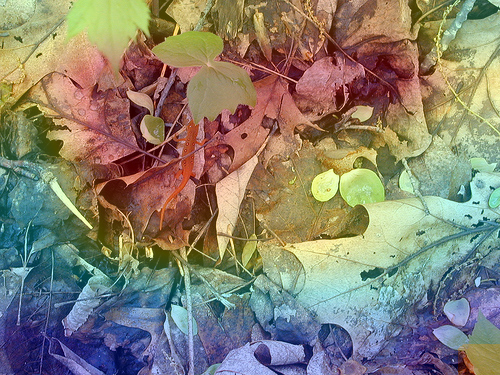
\includegraphics[width=3.5cm, height=3.0cm]{figures/robust_figure2.png}}
		\centerline{(1b) Q=15}
	\end{minipage}
	\hfill
	\begin{minipage}{0.2\linewidth}
		\centerline{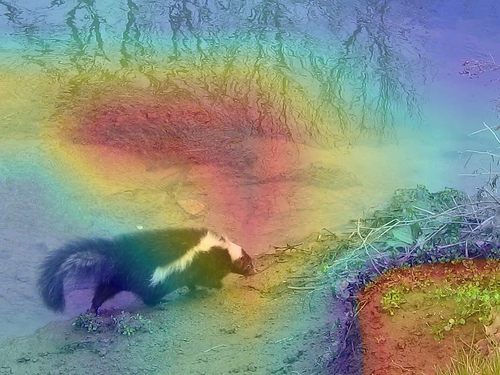
\includegraphics[width=3.5cm, height=3.0cm]{figures/robust_figure3.png}}
		\centerline{(1c) Q=15}
	\end{minipage}
	\hfill
	\begin{minipage}{0.2\linewidth}
		\centerline{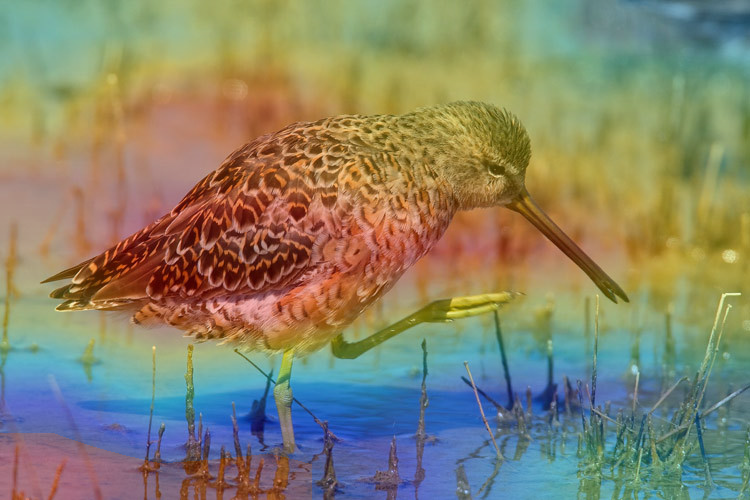
\includegraphics[width=3.5cm, height=3.0cm]{figures/robust_figure4.png}}
		\centerline{(1d) Q=15}
	\end{minipage}
	
	\vfill
	\vspace{0.4cm}
	
	\begin{minipage}{0.2\linewidth}
		\centerline{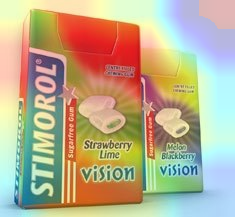
\includegraphics[width=3.5cm, height=3.0cm]{figures/sensetive_figure1.png}}
		\centerline{(2a) Q=85}
	\end{minipage}
	\hfill
	\begin{minipage}{0.2\linewidth}
		\centerline{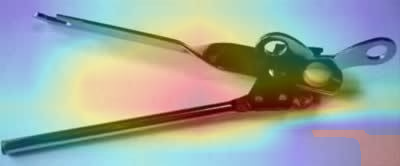
\includegraphics[width=3.5cm, height=3.0cm]{figures/sensetive_figure2.png}}
		\centerline{(2b) Q=85}
	\end{minipage}
	\hfill
	\begin{minipage}{0.2\linewidth}
		\centerline{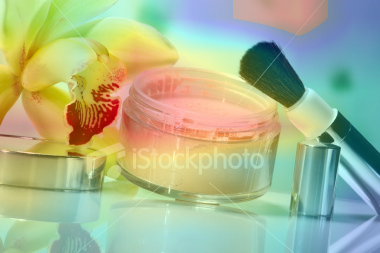
\includegraphics[width=3.5cm, height=3.0cm]{figures/sensetive_figure3.png}}
		\centerline{(2c) Q=75}
	\end{minipage}
	\hfill
	\begin{minipage}{0.2\linewidth}
		\centerline{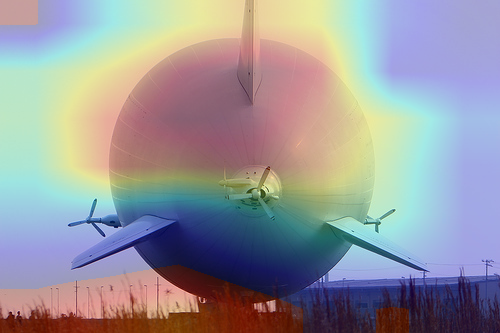
\includegraphics[width=3.5cm, height=3.0cm]{figures/sensetive_figure4.png}}
		\centerline{(2d) Q=75}
	\end{minipage}
%	\vspace{0.2cm}
	\caption{Visualization of the importance map for the RL agent to choose a compression quality level}
	\label{fig: attention}
\end{figure*}

In our investigations, we find that in different environments $ \{\mathcal{X}, M\} $, the RL agent selects compression quality levels based on the visual textures of different regions in the image. As shown in Figure~\ref{fig: attention}, picture 1a -- 1d are some pictures which the agent chooses to compress aggressively. The agent selects low compression quality levels based on the complex texture of the images. On the contrary, for pictures 2a -- 2d, the agent chooses relatively higher compression quality levels to preserve more details since its interest falls on some smooth regions. Especially for 1a and 2a, for picture 1a, the agent chooses a low compression quality level based on the rough central region though there are smooth regions around it, for picture 2a, the agent chooses a relatively higher compression quality level based on the surrounding smooth region rather than the central region. %% \\
\section{Evaluation}
\label{Section: evaluation}

In this section, we present AdaCompress's behaviors and effectiveness by some real-world experiments. %% \\

\subsection{Experiment Setup}

We carry out real-world experiments to verify our solution's performance. We use a desktop PC with an NVIDIA 1080ti graphic card as the edge infrastructure. For the cloud-based deep learning services, we choose Baidu Vision, Face++ object detection services and Amazon Rekognition. In the experiments, we use two datasets mentioned before in Subsection~\ref{subsec:insight}. The ImageNet dataset indicates daytime scenery, and the FLIR Thermal Dataset indicates nighttime scenery. Some important hyperparameters in our experiments are given in Table ~\ref{tab: parameters}.

\begin{table*}[!t]
	\centering
	\caption{Experiment parameter}
	\label{tab: parameters}
	%     \begin{tabular}{llllll}
	\begin{tabular}{cccccc}
		\toprule
		Notation          & Value & & & Notation     & Value  \\ \midrule
		$c_{\rm ref}$ & 75    & & & $K$      & 1000   \\
		$\epsilon_{\min}$    & 0.02  & & & $p_0$    & 0.2    \\
		$\gamma$      & 0.95  & & & $\omega$ & -3   \\
		$ \mu_{\rm dec} $ & 0.99 & & & $ T $ & 5  \\
		$r_{\rm th}$  & 0.45   & & &   $ n  $  &  10      \\ 
		{\color{revise} $ \mathcal{A}_0 $} & {\color{revise}0.8} & & & {\color{revise}$ T_{\rm start} $} & {\color{revise}128} \\
		$ {\color{revise}\alpha} $ & {\color{revise}1} & & & {\color{revise}$ \beta $} & {\color{revise}0}  \\ \bottomrule
	\end{tabular}
	%	\vspace{-0.5cm}
\end{table*}

%\begin{table*}[!t]
%	\centering
%	\caption{Experiment parameter}
%	\label{tab: parameters}
%	%     \begin{tabular}{llllll}
%	\begin{tabular}{cccccc}
%		\toprule
%		Notation          & Value & & & Notation     & Value  \\ \midrule
%		$c_{\rm ref}$ & 75    & & & $K$      & 1000   \\
%		$\epsilon_{\min}$    & 0.02  & & & $p_0$    & 0.2    \\
%		$\gamma$      & 0.95  & & & $\omega$ & -3   \\
%		$ \mu_{\rm dec} $ & 0.99 & & & $ T $ & 5  \\
%		$r_{\rm th}$  & 0.45   & & &   $ n  $  &  10      \\ \bottomrule
%	\end{tabular}
%%	\vspace{-0.5cm}
%\end{table*}

\subsection{Dataset}

We use two datasets, the ImageNet dataset and the FLIR Thermal Dataset. The ImageNet dataset is a Large-Scale Hierarchical Image, in which each node of the hierarchy is depicted by hundreds and thousands of images. Its images are mostly taken in the daytime. Therefore we use it as a daytime scenery. Usually, a surveillance camera captures colored pictures in the daytime and gray-scaled thermal images in the night. Therefore we choose a thermal image dataset to act as a nighttime image dataset. The FLIR Thermal Dataset is such a dataset having more than 14000 images collected by thermal sensors.

We use the ImageNet dataset in size reduction and accuracy performance experiment, DeepN-JPEG comparative experiment and end-to-end latency simulation experiment. Moreover, we use ImageNet and the FLIR Thermal Dataset alternately to simulate the scenery change in the \emph{inference-estimation-querying-retraining} mechanism experiment.

\subsection{Metrics}
\label{subsec:metrics}

The default compression quality level for JPEG is usually $75$ \cite{pillow_benchmark,imgmin}. Therefore we regard this as a reference value $ c_{\rm ref} = 75 $ of the conventional benchmark.

In our experiments, we measure the compressed and reference image's file size to obtain the compression rate $ \Delta s $. Since we do not have the real ground truth label of an image, we use the output $ \vec{y}_{\rm ref} $ from a reference image as the ground truth label, and calculate the relative top-5 accuracy $ \mathcal{A} $ as the accuracy metric. The formula of $ \mathcal{A} $ is presented in Subsection~\ref{subsec: formulation}.

\subsection{Upload Image Size Overhead}

\begin{figure}[!t]
	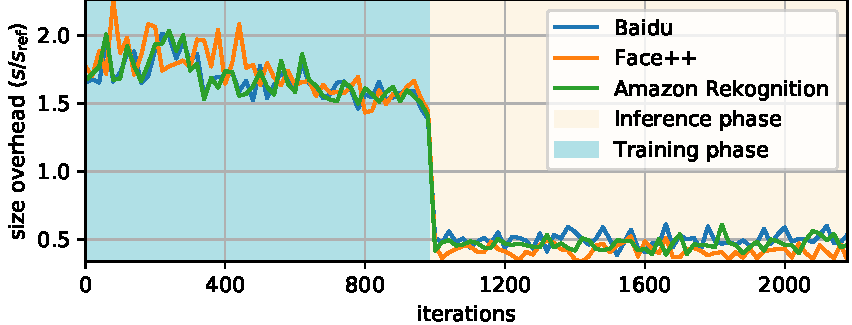
\includegraphics[width=0.8\linewidth]{figures/train_steps_new.pdf}
	\caption{Size overhead in the training and inference phase}
	\label{fig: train_steps}
	% \vspace{-0.3cm}
\end{figure}

Figure~\ref{fig: train_steps} presents the upload traffic load of the training and inference phase. To be more intuitionistic, we plot the size overhead {\color{revise2} $ \frac{\hat{s}}{\hat{s}_{\rm ref}} $} \iffalse $ \frac{s}{s_{\rm ref}} $ \fi as the $ y $-axis where {\color{revise2} $ \hat{s} $} is the real upload size of AdaCompress and {\color{revise2} $ \hat{s}_{\rm ref} $} is the benchmark upload size. Therefore $ y \geq 1 $ means that our solution uploads more data then benchmark, and $ y < 1 $ means the compression rate of AdaCompress. From Figure~\ref{fig: train_steps}, we can see that as the training procedure runs, the upload image size decreases because the RL agent learns to choose better compression quality levels to upload less data. In the training phase, to train the agent while remaining a convincing recognition result, AdaCompress has to upload the original image along with the compressed image to the cloud-end, obtaining the real result and the reward feedback. Therefore the upload traffic load is even higher than the conventional solution. But once the training phase has finished, the upload traffic load is lower than the benchmark. As shown in Figure~\ref{fig: compress_performance}, in the inference phase, AdaCompress's upload size is only 1/2 of the benchmark's. %% \\

\subsection{Size Reduction and Accuracy Performance}

\begin{figure}[!t]
	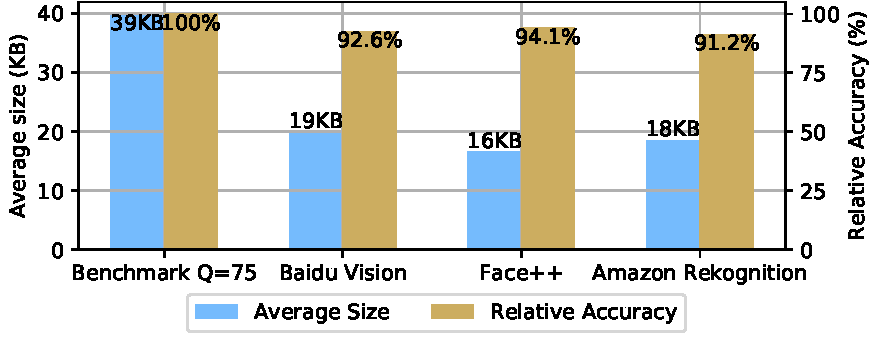
\includegraphics[width=0.8\linewidth]{figures/compress-performance.pdf}
	\caption{Average size and relative accuracy on different cloud services}
	\label{fig: compress_performance}
	% \vspace{-0.3cm}
\end{figure}

Figure~\ref{fig: compress_performance} presents the compression performance in the inference phase for each cloud service. We test AdaCompress on Face++, Baidu Vision and Amazon Rekognition. Comparing to the benchmark compression quality level, our solution can reduce the upload size by more than 1/2 for all tested cloud services, meanwhile maintain the relative accuracy that only decreases about 7\% on average, proving the efficiency of our design. %% \\

\subsection{DeepN-JPEG Comparative Experiment}

\begin{figure}[!t]
	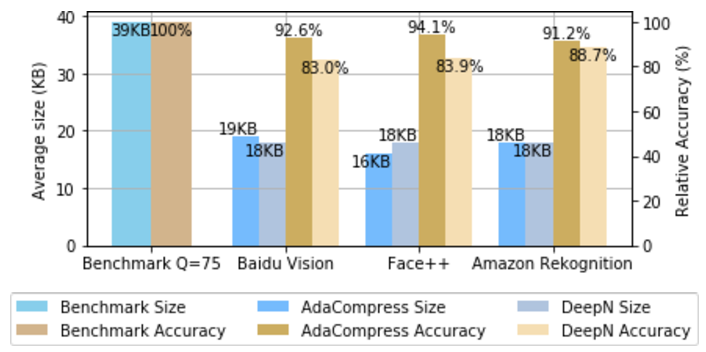
\includegraphics[width=0.8\linewidth]{figures/compare_DeepN.pdf}
	\caption{Comparative compression performance between DeepN-JPEG and AdaCompress}
	\label{fig: compare_DeepN}
	%    \vspace{-0.3cm}
\end{figure}

Figure~\ref{fig: compare_DeepN} presents a comparison performance between DeepN-JPEG and AdaCompress for each cloud service. As we can see, both DeepN-JPEG and AdaCompress cut down the upload size overhead more than 1/2. However, for all tested cloud services, AdaCompress's accuracy is higher than DeepN-JPEG's slightly. Compared with DeepN-JPEG's average accuracy is about 85\% on three cloud services, AdaCompress achieves a better average accuracy of 93\%. In a word, comparing to the DeepN-JPEG framework, AdaCompress presents a similar size reduction performance but achieving higher inference accuracy for online computer vision-based services.

\begin{figure*}[!t]
	\begin{minipage}{0.3\linewidth}
		\centerline{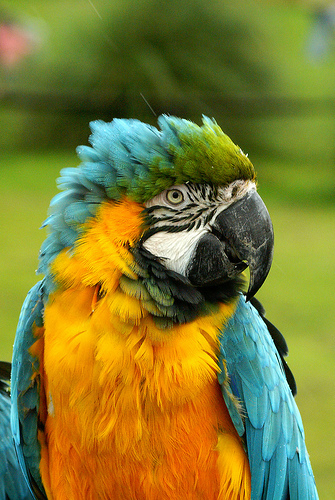
\includegraphics[width=4.0cm,trim=0 80 0 100,clip ]{figures/parrot_q75.jpeg}}
		\centerline{(1a) Origin Image (Q=75)}
		\centerline{Baidu prediction \ = \ [``parrot'']}
	\end{minipage}
	\hfill
	\begin{minipage}{0.2\linewidth}
		\centerline{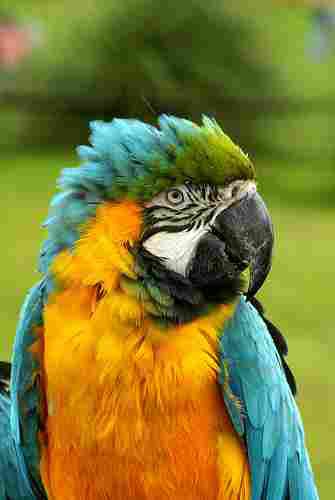
\includegraphics[width=4.0cm,trim=0 80 0 100,clip ]{figures/parrot_q15.jpeg}}
		\centerline{(1b) AdaCompress (choose Q=15)}
		\centerline{Baidu prediction \ = \ [``parrot'']}
	\end{minipage}
	\hfill
	\begin{minipage}{0.3\linewidth}
		\centerline{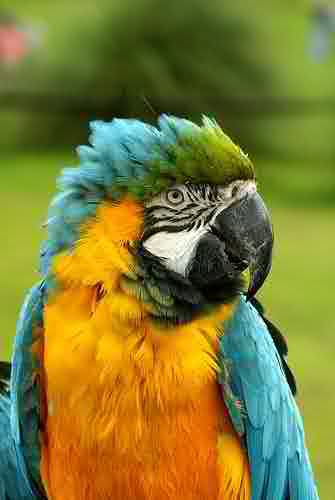
\includegraphics[width=4.0cm,trim=0 80 0 100,clip ]{figures/parrot_deepn.jpeg}}
		\centerline{(1c) DeepN-JPEG}
		\centerline{Baidu prediction \ = \ [``parrot'']}
	\end{minipage}
	
	\vfill
	\vspace{0.4cm}
	
	\begin{minipage}{0.3\linewidth}
		\centerline{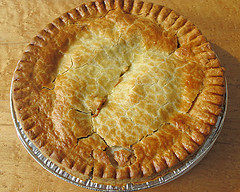
\includegraphics[width=4.0cm,trim=0 0 0 0,clip ]{figures/cake_q75.jpeg}}
		\centerline{(2a) Origin Image (Q=75)}
		\centerline{Baidu prediction \ = \ [``cake'']}
	\end{minipage}
	\hfill
	\begin{minipage}{0.2\linewidth}
		\centerline{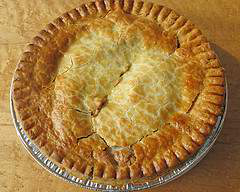
\includegraphics[width=4.0cm,trim=0 0 0 0,clip ]{figures/cake_q65.jpeg}}
		\centerline{(2b) AdaCompress (choose Q=65)}
		\centerline{Baidu prediction \ = \ [``cake'']}
	\end{minipage}
	\hfill
	\begin{minipage}{0.3\linewidth}
		\centerline{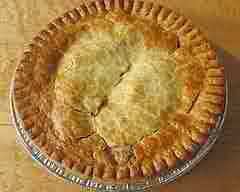
\includegraphics[width=4.0cm,trim=0 0 0 0,clip ]{figures/cake_deepn.jpeg}}
		\centerline{(2c) DeepN-JPEG}
		\centerline{Baidu prediction \ = \ [``fossil'']}
	\end{minipage}
	%	\vspace{0.2cm}
	\caption{Comparative compressed images of DeepN-JPEG and AdaCompress}
	\label{fig: compare_image}
\end{figure*}

AdaCompress compresses images in a more adaptive manner rather than DeepN-JPEG. (i.e., the explanation why AdaCompress achieves a better accuracy). As shown in Figure~\ref{fig: compare_image}, for picture 1a, compared to DeepN-JPEG, AdaCompress compresses the image at a more aggressive compression quality level of 15, reducing upload size overhead. On the contrary, for picture 2a of Figure~\ref{fig: compare_image}, DeepN-JPEG compresses the image with the same quantization table, but AdaComperss chooses a relatively higher compression quality level to preserve more details so that the backend deep learning model can still recognize the picture. Compared with DeepN-JPEG compresses all images with the same quantization table, AdaCompress chooses a low compression quality level for picture 1a and a relatively higher compression quality level for picture 2a based on the features of the input image. 

%Comparing to DeepN-JPEG, AdaCompress compresses images more adaptively for different images and cloud computer vision services to achieve higher accuracy, while maintaining a similar average upload size overhead.

Comparing to DeepN-JPEG, AdaCompress has two advantages and one disadvantage as following: %% \\    

\begin{itemize}
	
\item AdaCompress and DeepN-JPEG both decrease the upload size overhead more than 1/2, but AdaCompress maintains higher inference accuracy.

%\item DeepN-JPEG requires the original dataset information to re-design the quantization table, while AdaCompress chooses compression quality levels adaptively without any prior knowledge of the original dataset.
%\item When the scenery changes, DeepN-JPEG still compresses images with the same quantization table, while AdaCompress's \emph{inference-estimation-querying-retraining} mechanism captures the scenery change and make a more suitable compression strategy for the current scenery.
\item For different ``sceneries'' or cloud services, DeepN-JPEG compresses images with the same quantization table, while AdaCompress makes a more proper compression strategy adaptively.

%\item For different cloud services, DeepN-JPEG compresses images with the same quantization table, while AdaCompress makes a more proper compression strategy adaptively.
\item DeepN-JPEG re-designs the quantization table \emph{locally}, while AdaCompress needs to upload reference images and compressed images to the cloud-end in the training phase, leading some upload size overhead at the beginning. 
\end{itemize}

\subsection{Adaptively Cope With the Scenery Change}

To evaluate the efficiency of the \emph{inference-estimation-querying-retraining} mechanism, we feed AdaCompress with a combined dataset whose first 2000 images from FLIR Thermal images, the next 3000 images randomly sampled from ImageNet and the last 2000 images from FLIR Thermal images. We adapt AdaCompress's current RL agent to FLIR nighttime scenery by training it on the FLIR dataset, and run AdaCompress on the combined dataset, observing AdaCompress's behaviors upon the scenery changes at step 2000 and 5000. %% \\

We illustrate AdaCompress's behaviors in Figure~\ref{fig: running-retrain}. The $ x $-axis indicates steps, and the reference line indicates the scenery change. We plot AdaCompress's overall accuracy and the estimation probability $ p_{\rm est} $. At the bottom of Figure~\ref{fig: running-retrain}, we also plot the scaled upload size of AdaCompress and benchmark solution to illustrate the upload size overhead.
%with a $ \Delta $ mark on $ x $-axis

%\begin{figure}[!t]
%    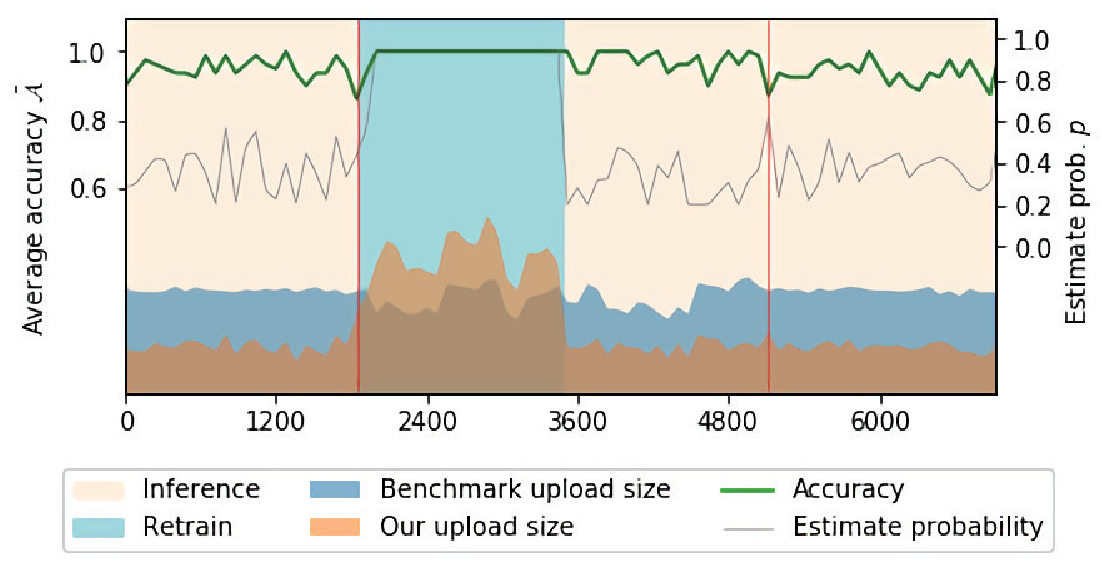
\includegraphics[width=\linewidth]{figures/running-retrain.pdf}
%    \caption{AdaCompress's reaction upon scenery change}
%%    \vspace{-0.2cm}
%    \label{fig: running-retrain}
%\end{figure}
\begin{figure}[!t]
	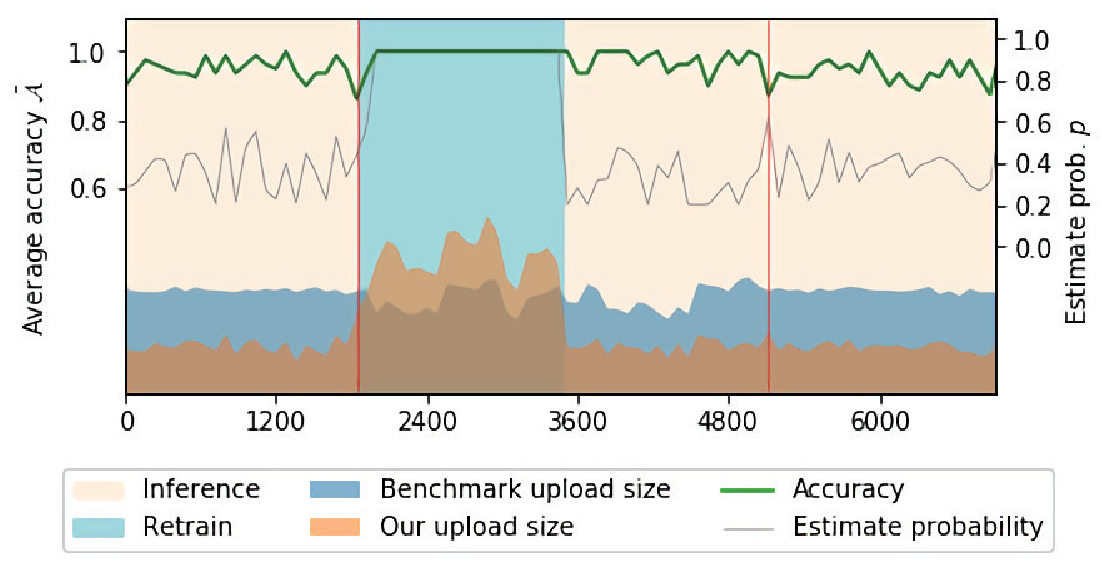
\includegraphics[width=0.8\linewidth]{figures/running-retrain.pdf}
	\caption{AdaCompress's reactions upon scenery change}
	%    \vspace{-0.2cm}
	\label{fig: running-retrain}
\end{figure}

From Figure~\ref{fig: running-retrain}, we can see that AdaCompress can adaptively update the estimation probability $ p_{\rm est} $. When the overall accuracy decreases, AdaCompress would increase the estimation probability, trying to capture the scenery change. When the overall accuracy is stable and high enough, the estimation probability $ p_{\rm est} $ decreases to reduce transmission. %% \\

Upon the first image scenery changes (i.e., night to day) shown as the first reference line in Figure~\ref{fig: running-retrain}, comparing to the earlier steps, the accuracy decreases dramatically and the estimation probability $ p_{\rm est} $ raises to determine whether the scenery changes. The accuracy keeps dropping in the following steps, indicating that the current RL agent is no more suitable for the current input scenery. At the moment, AdaCompress should switch to the model querying state and re-load a new RL agent model from the model caching library. However, there is no model except the current RL agent at that time. Therefore, AdaCompress starts to re-train at once to adapt the RL agent to the current scenery. In the re-training phase, AdaCompress uses the reference image's prediction label $ \vec{y}_{\rm ref} $ as the output result. Therefore the accuracy $ \mathcal{A} $ and $ p_{\rm est} $ are locked to 1. After finishing re-training the agent in the daytime scenery, the trained agent is cached in the model caching library. In the following steps, sometimes the accuracy decreases accidentally, and the estimation probability $ p_{\rm est} $ also raises. The accuracy is not lower than the accuracy threshold $ \mathcal{A}_0 $. Therefore the re-training phase would not be triggered again until the second image scenery changes. %% \\

Upon the second image scenery changes (i.e., day to night) shown as the second reference line in Figure~\ref{fig: running-retrain}, like the first scenery change, the accuracy decreases and $ p_{\rm est} $ raises, indicating that the current RL agent is no more suitable again. AdaCompress switches to the model querying state at once and re-loads a new RL agent model (the initial model trained on the FLIR Thermal images) from the model caching library. When using the new agent in this scenery, the accuracy stops decreasing and maintains more than the accuracy threshold, indicating the current RL agent is suitable for the current scenery.  %% \\

From Figure~\ref{fig: running-retrain}, we can also observe the upload size overhead in different phases. In the re-training phase, AdaCompress uploads more data than the conventional benchmark. But in the inference phase, AdaCompress's upload size is only half of the benchmark's. Especially once the second image scenery changes, AdaCompress achieves a low upload traffic load by re-loading a suitable RL agent model rather than re-training from scratch. %% \\

\subsection{End-to-End Latency Simulation}

Comparing to the conventional solution that uploads the image directly, in our solution, the image is passed to the RL agent firstly to estimate the compression quality level. Running this RL agent brings extra latency to the whole system. In this subsection, we evaluate the end-to-end latency. %% \\

We compute compressed file size for batches of images, and test the RL agent's inference time and the latency of uploading such compressed images. \textcolor{revise}{We respectively test the average inference latency on 1000 ImageNet images and 1000 FLIR images}, and simulate the network bandwidth as 27.64 Mbps according to the global average fixed broadband upload speed~\cite{speedtest} in Feb. 2019, to verify the end-to-end latency performance. The latency comparison is listed in Table~\ref{tab: latency-overhead}. %% \\

%We compute compressed file size for batches of images, and test the RL agent's inference time and the latency of uploading such compressed images. We test the average inference latency on 1000 ImageNet images and simulate the network bandwidth as 27.64 Mbps according to the global average fixed broadband upload speed~\cite{speedtest} in Feb. 2019, to verify the end-to-end latency performance. The latency comparison is listed in Table~\ref{tab: latency-overhead}. %% \\

\begin{table*}[!t]
{\color{revise}
	\centering
	\caption{\textcolor{revise}{Latency of edge device to cloud service}}
	\label{tab: latency-overhead}
	%     \begin{tabular}{lll}
	\resizebox{\textwidth}{!}{
	\begin{tabular}{cccccc}
		\toprule
		Dataset & Solution & Average upload size & Inference latency \
		& Transmission latency & End-to-end latency \\ \midrule
		ImageNet & Benchmark & 42.68 KB & 0 ms & 12.35 ms & 12.35 ms \\
		ImageNet & AdaCompress & 18.64 KB & 2.09 ms & 5.34 ms & 7.43 ms \\
		FLIR & Benchmark & 44.66 KB & 0 ms & 12.93 ms & 12.93 ms \\
 		FLIR & AdaCompress & 17.07 KB & 2.03 ms & 4.94 ms & 6.97 ms \\ \bottomrule
	\end{tabular}}
	% \vspace{-0.5cm}
}
\end{table*}
%\begin{table*}[!t]
%	\centering
%	\caption{Latency between image upload and inference result feedback}
%	\label{tab: latency-overhead}
%	%     \begin{tabular}{lll}
%	\begin{tabular}{ccc}
%		\toprule
%		& Benchmark & AdaCompress  \\ \midrule
%		Average upload size          & 42.68 KB  &  18.46 KB            \\
%		Inference latency    & 0 s       & 2.09 ms          \\
%		Transmission latency & 12.35 ms       & 5.34 ms          \\
%		Overall latency      & 12.35 ms       & 7.43 ms          \\ \bottomrule
%	\end{tabular}
%	% \vspace{-0.5cm}
%\end{table*}

Our solution brings in inference latency to the end-to-end latency, but the transmission latency is low by reducing the upload file size. In today's network architecture where the edge infrastructure's computational power is increasing significantly~\cite{satyanarayanan2017emergence,hu2015mobile}, we can use the computing power of the edge infrastructure in exchange for the reduction of upload traffic load and transmission latency. \textcolor{revise}{Compared with the benchmark solution, our solution effectively reduces the end-to-end latency on both ImageNet and FLIR dataset.} %% \\

\subsection{\textcolor{revise}{Overall Memory and Latency Overhead}}

\subsubsection{\textcolor{revise}{Memory Overhead:}}
\textcolor{revise}{The memory overhead is divided into two parts: the static occupied memory space and dynamic memory usage. Firstly, the static occupied memory space is the memory of the model's size. We use Keras to construct and save MobileNetV2 and the RL agent. We check file size of the saved model as the model's size. A RL agent model's size is 1 MB, and the feature extractor MobileNetV2's size is 8.9 MB. The model caching library stores the most recent five RL agents. The overall memory of the model's size is at most 13.9 MB. Secondly, the dynamic memory usage is the memory usage during AdaCompress runs. The overall memory usage mainly includes the memory buffer of transitions and the memory usage caused by the RL agent and feature extractor. When caching transitions of 1000 images in the memory buffer, it occupies about 500 KB. We use Psutil to measure the peak memory usage during AdaCompress runs. The peak memory usage is about 367 MB. Thirdly, in real-world edge-application scenarios, common edge infrastructures have enough memory to deploy this algorithm, such as Raspberry Pi 4 Model B's \cite{Raspberry-Pi} memory is 2/4/8 GB, and Huawei Atlas 500 edge station's memory is 4/8 GB.}

\subsubsection{\textcolor{revise}{Training and Re-loading Latency:}}
\textcolor{revise}{Although AdaCompress can be highly efficient to run on today's edge infrastructures, it would cause extra latency overhead, such as training and re-loading latency. In this subsection, we evaluate the latency overhead.}

%\begin{table*}[!t]
%	\centering
%	\caption{Time cost of training}
%	\label{tab: training-time}
%		\begin{tabular}{cccc}
%			\toprule
%			Dataset & Number of training images & Time cost & Real time cost \\ \midrule
%			ImageNet & 898 & 15.86 min & 7.89 min \\
%			FLIR & 910 & 15.63 min & 7.85 min \\ \bottomrule
%	\end{tabular}
%	% \vspace{-0.5cm}
%\end{table*}

\textcolor{revise}{In our experiments, the convergence condition of training is that the recent average accuracy over 0.8 meanwhile the recent average reward over 0.45. The experiment results show the number of training images is 898 and 910 on ImageNet and FLIR, respectively. The time cost mainly depends on the frequency of sending images and the inference speed of the cloud service. If the end-user sends images continuously, and cloud service's inference speed is about 10 images per second, the time costs are 197.3s and 200.8s on ImageNet and FLIR, respectively. In the training phase, we need to upload reference images and compressed images. We consider the time cost of uploading reference images and obtaining the feedbacks as the benchmark latency. If we minus this benchmark latency, the real training time cost is not over 100s. It is worth to spend such upload size overhead and time cost at the beginning when we need to infer thousands of images.}

%And the training time respectively is 15.36 min and 15.63 min on ImageNet and FLIR.

\textcolor{revise}{The \emph{inference-estimation-querying-retraining} mechanism would either re-load or re-train a RL agent intelligently when capturing the scenery change. The re-training time cost is similar to the training time cost which is described above. The latency of re-loading a RL agent model is about 1.85s. To \emph{reduce} this latency, we use another process to re-load the model in our experiments. The mechanism still uses the old RL agent to choose a compression quality level before the re-loading process has finished.}

%\input{sections/related_works}
\section{Conclusion}
\label{Section: conclusion}

To reduce the upload traffic load of deep learning applications, most researchers focus on modifying the deep learning model, but this does not apply to the industry because the backend deep learning model is usually inaccessible to users. We present a heuristic solution using a reinforcement learning agent to decide the proper compression quality level for each image according to the image's features and the backend service. Our experiment results show that for different backend deep learning cloud services and different input image ``sceneries'', using different compression strategies can significantly reduce the upload file size overhead while keeping comparable accuracy. Moreover, we design the \emph{inference-estimation-querying-retraining} mechanism to cope with the input image scenery change and make a proper compression strategy for the current scenery. Our experiment results show that once the scenery changes, the mechanism would either re-load a pre-trained agent or re-train a new agent intelligently to achieve low upload image size overhead while maintaining the inference accuracy.


%\begin{acks}
%To Robert, for the bagels and explaining CMYK and color spaces.
%\end{acks}

\bibliographystyle{ACM-Reference-Format}
%\bibliography{sample-base}
\bibliography{main}

%%
%% If your work has an appendix, this is the place to put it.
%\appendix

\end{document}
\endinput
%%
%% End of file `sample-acmsmall.tex'.
